
\documentclass[oneside,intlimits,reqno]{scrbook}

%% PACKAGES -------------------------------------------------------------------------------------
\usepackage{array}
\usepackage{enumerate}
\usepackage{mathrsfs}
\usepackage{mathtools}
\usepackage{pgf,tikz}
\usetikzlibrary{arrows}
\usepackage{extarrows}
\usepackage{graphicx,makeidx}
\usepackage{a4wide}
\usepackage{ragged2e}
\usepackage[nottoc]{tocbibind}
\usepackage{amsmath,amssymb,amsthm,amsfonts}
\usepackage{mathabx}
\usepackage[utf8]{inputenc}
\usepackage[czech]{babel}
\usepackage{relsize}
\usepackage[unicode,breaklinks=true,hypertexnames=false]{hyperref}
\def\dotminus{\mathbin{\ooalign{\hss\raise1ex\hbox{.}\hss\cr
			\mathsurround=0pt$-$}}}

%% DEFINICE A REDEFINICE ZÁKLADNÍCH PŘÍKAZŮ ------------------------------------------------------
%definice textu nad rovnítkem
\newcommand{\equal}[1]{\mathop{\overset{#1}{\resizebox{\widthof{.{\ensuremath{\mathop{\overset{#1}{\mathop{=}}}}.}}}{\heightof{=}}{$\mathop{=}$}}}}

% redefinice znaků
\renewcommand{\epsilon}{\varepsilon}
\let\crossedphi\phi
\renewcommand{\phi}{\varphi}
\renewcommand{\rho}{\varrho}
\renewcommand{\emptyset}{\font\cmsy = cmsy10 at 12pt\hbox{\cmsy \char 59}}

% definice českých uvozovek
\def\bq{\mbox{\kern.1ex\protect\raisebox{-1.3ex}[0pt][0pt]{''}\kern-.1ex}}
\def\eq{\mbox{\kern-.1ex``\kern.1ex}}
\gdef\uv#1{\bq #1\eq}

%% MATEMATIKA ----------------------------------------------------------------------------------
% konstanty atd.
\renewcommand{\d}{\mathrm{d}} % diferenciál
\newcommand{\me}{\mathrm{e}} % eulerovo číslo
\newcommand{\mi}{\mathrm{i}} % imaginární jednotka
\newcommand{\LL}{\mathscr{L}}
\newcommand{\Loss}{\mathscr{L}}

% matematické výrazy
\newcommand{\tg}{\mathop{\mathrm{tg}}}				% tangens
\newcommand{\argmin}{\mathop{\mathrm{argmin}}}		% argmin	
\newcommand{\argmax}{\mathop{\mathrm{argmax}}}		% argmax
\newcommand{\argsup}{\mathop{\mathrm{argsup}}}		% argsup
\newcommand{\sgn}{\mathrm{sgn}}						% signum
\renewcommand{\Re}{\mathop{\mathrm{Re}}}
\newcommand{\Ran}{\mathop{\mathrm{Ran}}}
\newcommand{\supp}{\mathop{\mathrm{supp}}}			% support
\renewcommand{\Im}{\mathop{\mathrm{Im}}}
\newcommand{\trace}{\text{tr}} 						% stopa
\newcommand{\inv}[1]{{#1^{-1}}}

% množiny čísel
\newcommand{\R}{\mathbb{R}} % množina reálných čísel
\renewcommand{\C}{\mathbb{C}} % množina komplexních čísel
\newcommand{\Z}{\mathbb{Z}} % množina celých čísel
\newcommand{\N}{\mathbb{N}} % množina přirozených čísel


%% ZKRATKY ---------------------------------------------------------------------------
\newcommand{\MSE}{\mathrm{MSE}}
\newcommand{\MLE}{\mathrm{MLE}}
\newcommand{\LSE}{\mathrm{LSE}}
\newcommand{\MSR}{\mathrm{MSR}}
\newcommand{\NF}{\mathrm{F}}
\newcommand{\A}{\mathrm{A}}
\newcommand{\RMR}{\mathrm{R}}
\newcommand{\SST}{\mathrm{SST}}
\newcommand{\SSE}{\mathrm{SSE}}
\newcommand{\SSR}{\mathrm{SSR}}


% MATICE ------------------------------------------------------------------------------
 % indentita
\newcommand{\I}{\mathbb{I}} % identita
\newcommand{\Identita}[1]{\mathbb{I}_{#1}} % identita s indexem velikosti
% obecné matice A,B,H
\newcommand{\Am}{\mathbb{A}} % matice A
\newcommand{\Bm}{\mathbb{B}}
\newcommand{\Hm}{\mathbb{H}}
\newcommand{\Mm}{\mathbb{M}}
\newcommand{\Wm}{\mathbb{W}}
\newcommand{\Km}{\mathbb{K}}
% Fisherova matice
\newcommand{\fisher}{\mathbb{I}} % Fisherova matice





\newcommand{\Cc}{\mathcal{C}} % funkce třídy C (spojité)
\newcommand{\RR}{\mathcal{R}}



% VEKTORY ----------------------------------------------------------------------------------------------
% vektorová písmenka x,y,X,Y atd.
% tučné X
\newcommand{\X}{\textbf{X}} % klasické
\newcommand{\lX}{\overline{\textbf{X}}} % s pruhem
% tučné Y
\newcommand{\Y}{\textbf{Y}} % klasické
\newcommand{\lY}{\overline{Y}} % s pruhem
% tučné x
\newcommand{\x}{\textbf{x}}
% tučné y
\newcommand{\y}{\textbf{y}}
% tučné z
\newcommand{\z}{\textbf{z}}

% beta
\newcommand{\betab}{\boldsymbol{\beta}} 			% vektorové beta
\newcommand{\bbeta}{\boldsymbol{\beta}}				% také vektorové beta
\newcommand{\wbetab}{\widehat{\boldsymbol{\beta}}}	% vektorové beta se stříškou
% rezidua: e
\newcommand{\eb}{\textbf{e}}
\newcommand{\lei}{\overline{e}_i}
\newcommand{\hei}{\widehat{e}_i}
% epsilon
\newcommand{\epsb}{\boldsymbol{\epsilon}}


%% PROMĚNNÉ SE STŘÍŠKOU -----------------------------------------------------------------------------------
% řecká abeceda
\newcommand{\walpha}{\widehat{\alpha}}				% alpha se stříškou
\newcommand{\wbeta}{\widehat{\beta}}				% beta se stříškou
\newcommand{\wgamma}{\widehat{\gamma}}				% gamma se stříškou
\newcommand{\wsigma}{\widehat{\sigma}}				% sigma se stříškou
\newcommand{\heps}{\widehat{\epsilon}}				% epsilon se stříškou
\newcommand{\hrho}{\widehat{\rho}}
\newcommand{\wtheta}{\widehat{\theta}}
% x se stříškou
\newcommand{\hxn}{\widehat{x}_n}	% xn se stříškou
% y se stříškou
% klasické
\newcommand{\hy}{\widehat{y}}
\newcommand{\hY}{\widehat{Y}}
% z se stříškou
\newcommand{\hz}{\widehat{z}}
\newcommand{\hzb}{\widehat{\z}}
% s indexy
\newcommand{\hyn}{\widehat{y}_n}
\newcommand{\hyi}{\widehat{y}_i}
\newcommand{\hYn}{\widehat{Y}_n}
\newcommand{\hYi}{\widehat{Y}_i}
% vektorové
\newcommand{\hYb}{\widehat{\textbf{Y}}}
\newcommand{\hyb}{\widehat{\textbf{y}}}
% rezidua: e
\newcommand{\he}{\widehat{e}}
\newcommand{\heb}{\widehat{\textbf{e}}}
% a nějaké další
\newcommand{\hsn}{\widehat{\sigma}_n^2}				% sn se stříškou


%% PROMĚNNÉ S PRUHEM --------------------------------------------------------------------------------------
\newcommand{\overbar}[1]{\mkern 1mu\overline{\mkern-1mu#1\mkern-3mu}\mkern 3mu}
\newcommand{\Oxn}{\overbar{\rule{0ex}{1.8ex}X_n}}
\newcommand{\Oyn}{\overbar{\rule{0ex}{1.8ex}Y_n}}
\newcommand{\Ox}[1]{\overbar{\rule{0ex}{1.8ex}X_{#1}}}
\newcommand{\Oy}[1]{\overbar{\rule{0ex}{1.8ex}Y_{#1}}}
\newcommand{\oxn}{\overbar{\rule{0ex}{1.33ex}X_n}}
\newcommand{\ox}[1]{\overbar{\rule{0ex}{1.33ex}X_{#1}}}
\newcommand{\oy}[1]{\overbar{\rule{0ex}{1.33ex}Y_{#1}}}
\newcommand{\oyn}{\overbar{\rule{0ex}{1.33ex}Y_n}}
\newcommand{\omn}{\overbar{\rule{0ex}{1.3ex}\mu_n}}
\newcommand{\oxnn}{\overbar{\rule{0ex}{1.33ex}x_n}}
\newcommand{\oynn}{\overbar{\rule{0ex}{1.33ex}y_n}}

% další možnost
\newcommand{\lyn}{\overline{y}_n}
\newcommand{\ly}{\overline{y}}
\newcommand{\lhyn}{\overline{\hy}_n}
\newcommand{\lhy}{\overline{\hy}}
\newcommand{\lyi}{\overline{y}_i}
\newcommand{\lxn}{\overline{x}_n}
\newcommand{\lx}{\overline{x}}


%% PRAVDĚPODOBNOST ------------------------------------------------------------------------------
% distribuční funkce
\newcommand{\FF}{\mathrm{F}}
\newcommand{\FEX}{\FF_\X}

% hustota pravděpodobnosti
\newcommand{\fex}{f_\X}

% pravděpodobnost
\newcommand{\PP}{\mathbb{P}}
\newcommand{\PEX}{\PP^\X}

% pravděpodobnostní prostor
\newcommand{\prostor}{(\Omega,\mathcal{A},\PP)} 

% charakteristiky
\newcommand{\E}{\mathbb{E}} % střední hodnota
\newcommand{\D}{\mathrm{D}} %  rozptyl
\newcommand{\Cov}{\mathbb{C}\mathrm{ov}} % kovariance

% rozdělení
\newcommand{\NN}{\mathcal{N}} % normální
\newcommand{\AN}{\mathcal{AN}} % asymptoticky normální
\newcommand{\Exp}{\mathrm{Exp}} % exponenciální
\newcommand{\Be}{\mathrm{Be}} % bernoulliho
\newcommand{\Bi}{\mathrm{Bi}} % binomické

% konvergence
\newcommand{\sj}{\stackrel{s.j.}{\longrightarrow}}
\newcommand{\Pto}{\stackrel{\PP}{\to}}
\newcommand{\wto}{\stackrel{w}{\to}}
\newcommand{\Dto}{\stackrel{\mathscr{D}}{\to}}
\newcommand{\PSJ}{\stackrel{\PP,s.j.}{\longrightarrow}}
\newcommand{\Lto}{\stackrel{(\mathscr{L})}{\to}}
\newcommand{\sjP}{\stackrel{s.j.~\PP}{\longrightarrow}}
\newcommand{\Lp}{\stackrel{L_p}{\longrightarrow}}

% pár dalších...
\newcommand{\Aa}{\mathcal{A}}
\newcommand{\Bb}{\mathcal{B}}
\renewcommand{\t}{\theta} % theta
\newcommand{\bmu}{\boldsymbol{\mu}} % vektorové mí

\newcommand{\htm}{\widehat{\t}_\txt{M}}
\newcommand{\html}{\widehat{\t}_\txt{ML}}
\newcommand{\htn}{\widehat{\t}_n}
\newcommand{\rhn}{R_{H_0}}
\newcommand{\Phiast}{\crossedphi^\ast}
\newcommand{\rhno}{\overline{R}_{H_0}}
\newcommand{\freg}{\mathcal{F}_{reg}}
\newcommand{\fregp}{\mathcal{F}_{reg}^+}
\newcommand{\fregml}{\mathcal{F}_{reg}^\txt{ML}}
\newcommand{\RE}{\mathrm{RE}_{2,1}}
\newcommand{\ARE}{\mathrm{ARE}_{2,1}}

% proměnné s dolním složitějším indexem
\newcommand{\hii}{h_{ii}}
\newcommand{\Sxx}{ S_{xx} }

% co moc nikam nepatří...
\newcommand{\core}{\inv{(\textbf{X}^T\textbf{X})}}
\newcommand{\lomn}[1]{\frac{#1}{n}}
\newcommand{\lm}{\frac{1}{m}}
\newcommand{\jednab}{\mathbf{1}}
\newcommand{\norm}[1]{\| #1 \|}
\newcommand{\In}{\mathrm{I}_n}
\newcommand{\Q}{\textbf{Q}}



%% POSLOUPNOSTI, SUMY ATD. -------------------------------------------------------------------------------------
%posloupnosti
\newcommand{\posl}{(X_j)_{j=1}^{+\infty}}
\newcommand{\poslkon}{(X_j)_{j=1}^{n}}
\newcommand{\posln}{(X_n)_{n=1}^{+\infty}}
\newcommand{\poslnn}{(\X_n)_{n=1}^{+\infty}}

%sumy
\newcommand{\suminftyo}{\sum\limits_{n=0}^{+\infty}}
\newcommand{\suminfty}{\sum\limits_{n=1}^{+\infty}}
\newcommand{\sumainfty}[1]{\sum\limits_{#1}^{+\infty}}
\newcommand{\suminftylo}{\sum\limits_{l=0}^{+\infty}}
\newcommand{\sumin}{\sum\limits_{i=1}^{n}}
\newcommand{\sumjn}{\sum\limits_{j=1}^{n}}
\newcommand{\sumjm}{\sum_{j=1}^{m}}
\newcommand{\sm}[2]{\sum\limits_{ #1 }^{ #2 }}


%% NĚJAKÉ DALŠÍ PŘÍKAZY -----------------------------------------------------------------------------------------
\newcommand{\dom}[1]{\mathop{\mathrm{Dom} (#1)}} % definiční obor
\newcommand{\mat}[1]{\mathbf #1}
\newcommand{\abs}[1]{\left|#1\right|}
\renewcommand{\b}[1]{\left( #1 \right)}
\newcommand{\nor}[1]{\left\|#1\right\|}
\newcommand{\Br}[1]{\Bigl(#1\Bigr)}
\newcommand{\br}[1]{\bigl(#1\bigr)}
\newcommand{\e}[1]{\me^{#1}}
\newcommand{\mini}[1]{{#1_{(-1)}}}
\newcommand{\ini}{\theta\in\Theta}
\newcommand{\init}[1]{\theta\in\Theta\subset\R^#1}
\newcommand{\txt}[1]{\mathrm{{\footnotesize  #1 }}}
\newcommand{\matice}[4]{\left(\begin{array}{cc}	#1 & #2 \\ #3 & #4	\end{array} \right)}
\newcommand{\maticehrana}[4]{\left[\begin{array}{cc}	#1 & #2 \\ #3 & #4	\end{array} \right]}
\newcommand{\vektor}[2]{\left(\begin{array}{c}	#1  \\  #2	\end{array} \right)}
\newcommand{\p}[1]{\PP\left( #1 \right)}
\newcommand{\EE}[1]{\E\left[ #1 \right]}
\newcommand{\n}[1]{\NN\left( #1 \right)}
\newcommand{\hypothesis}[2]{H_0: #1 ~\text{vs.}~ H_1: #2 }
\newcommand{\hypothesiswide}[2]{H_0: #1 \qquad\text{vs.}\qquad H_1: #2 }
\newcommand{\silofunkce}[1]{\beta_\crossedphi\big|_{\Theta_{#1}}}
\newcommand{\silofunkceast}[1]{\beta_{\Phiast}\big|_{\Theta_{#1}}}
\newcommand{\hypothesisap}[2]{H'_0: #1 ~\text{vs.}~H'_1: #2 }
\newcommand{\test}[1]{\boxed{\text{TEST: $H_0$ zamítáme, pokud } #1 .}}
\renewcommand{\S}{\mathbb{S}}


%% PROSTŘEDÍ -----------------------------------------------------------------------------------------------------
\theoremstyle{definition}
\newtheorem{define}{Definice}[chapter]
\theoremstyle{plain}
\newtheorem{theorem}[define]{Věta}
\newtheorem{lemma}[define]{Lemma}
\newtheorem{dusl}[define]{Důsledek}
\newtheorem{corollary}[define]{Tvrzení}
\renewcommand{\proofname}{Důkaz}

\theoremstyle{remark}
\newtheorem{example}[define]{\textsc{Příklad}}
\newtheorem{remark}[define]{\textsc{Poznámka}}

\renewcommand{\indexname}{Rejstřík}

\frenchspacing
\setlength{\parindent}{0pt}
\setlength{\parskip}{1pt}

\hypersetup{
 	pdftitle={01RAD - Regresní analýza dat},
 	pdfauthor={WIKI Skripta},
 	pdfsubject={Zápisky z přednášek RAD, FJFI ČVUT},
 	pdfkeywords={regresní analýza dat},
 	bookmarksnumbered=true,
 	colorlinks=true,
 	pdfpagemode={UseOutlines}
 }
\makeindex

\title{01RAD}
\date{\today}
\author{doc.~Ing.~Tomáš Hobza,~Ph.D., Martin Kovanda, Michaela Mašková, Filip Bár}

\begin{document}

% ****************************************************************************************************************************
%                             FRONTMATTER
% ****************************************************************************************************************************
\frontmatter
\maketitle

\newpage
\pdfbookmark[0]{Obsah}{obsah}
\tableofcontents

%\wikiskriptum{01DIFRnew}
% ****************************************************************************************************************************
%                             KAPITOLA: Předmluva
% ****************************************************************************************************************************
\chapter*{Předmluva}
\pdfbookmark[0]{Předmluva}{predmluva}

Materiál byl sestaven na základě poznámek doc. Ing. Tomáše Hobzy, Ph.D., kterému bychom tímto chtěli poděkovat za rozsáhlou korekci vzniklého materiálu. Zmíněné přednášky proběhly v~zimním semestru akademického roku 2020/2021 na~Fakultě jaderné a
fyzikálně inženýrské ČVUT v~Praze. Přednášky nebyly uskutečněny prezenční formou vzhledem k probíhající pandemii Covid-19. 

Tento učební text je určen posluchačům 1.~ročníku navazujícího magisterského studia navštěvujícím kurs 01RAD\emph{	Regresní analýza dat}, který je zařazen
mezi předměty oborů AMSM. Při sestavování textu se předpokládaly znalosti základů matematiky na úrovni absolvování kurzů 01MAB2-4, 01LAB1-2 a 01MIP.

~

\textbf{Doporučená literatura:}
\begin{enumerate}[(1)]
  \item ...
\end{enumerate}



% ****************************************************************************************************************************
%                             MAINMATTER
% ****************************************************************************************************************************
\mainmatter
%regresní analýza
\chapter{Opakování ze SME}
\section{Jednorozměrná lineární regrese}
%příklad matlab
Předpokládejme, že se~sledují dvě fyzikální veličiny $X$ a~$Y$ mezi~kterými existuje lineární závislost
$$Y=\beta_0+\beta_1X .$$
$\beta_0$ a~$\beta_1$ nejsou známy, a~proto se~provádí experiment, při~němž se~zjišťují hodnoty dvojic $(X,Y)$. Často se~stává, že měření hodnot $X$ probíhá prakticky zcela přesně (například $X$ se~nastavuje na~předem dané úrovně), zatímco $Y$ se~měří s~určitou chybou. Zavádí se~tedy model
$$Y_i=\beta_0 +\beta_1X_i + e_i \quad \forall~i=1,...,n,$$
kde $e_i$ je náhodný šum a~$e_1,...,e_n$ jsou $iid~\NN(0,{\sigma}^2)$ a~dvojice $(x_1,y_1),...,(x_n,y_n)$ získáme měřením. Neznáme parametry jsou $\beta_0,\beta_1, {\sigma}^2$, chtěli bychom je odhadnout na~základě výběru (MLE odhady).\\

Rozdělení $Y_i$ je $Y_i\sim\NN(\beta_0 + \beta_1x,{\sigma}^2)$, a~tedy věrohodnostní funkce výběru $y_1,...,y_n$ je
$$L=\Br{\frac{1}{\sqrt{2\pi{\sigma}^2}}}^n \e{-\frac{1}{2{\sigma}^2}\sum_{i=1}^{n}(Y_i-\beta_0-\beta_1x)^2}.$$
$$l=\ln L=-\frac{n}{2}\ln{2\pi}-\frac{n}{2}\ln{{\sigma}^2}-\frac{1}{2{\sigma}^2}\sum_{i=1}^{n}(Y_i-\beta_0-\beta_1x_i)^2.$$
Je zřejmé, že pro~libovolné ${\sigma}^2$ potřebujeme minimalizovat
$$S(\beta_0,\beta_1)=\sum_{i=1}^{n}(Y_i-\beta_0-\beta_1x_i)^2   $$
přes $\beta_0,\beta_1$, na~což použijeme metodu nejmenších čtverců (poznámka?).
$$\frac{\partial l}{\partial \beta_0}=2\frac{1}{2{\sigma}^2}\sum_{i=1}^{n}(Y_i-\beta_0-\beta_1x_i)=0,  $$
$$\frac{\partial l}{\partial \beta_1}=\frac{1}{{\sigma}^2}\sum_{i=1}^{n}(Y_i-\beta_0-\beta_1x_i) x_i=0. $$
Z toho pak
$$  \sum_{i=1}^{n} Y_i -n\beta_0-\beta_1 \sum_{i=1}^{n} x_i=0, $$
$$ \beta_0=\Oyn -\beta_1\oxnn=\frac{1}{n}\sum_{i=1}^{n}Y_i-\beta_1\frac{1}{n}\sum_{i=1}^{n}x_i.$$
Po vynásobení poslední rovnice $n$ úpravou dostaneme vztah
$$\sum_{i=1}^{n}(Y_i-\Oyn+\beta_1\oxnn-\beta_1x_i)x_i=0  $$
a následně i~vztah
$$ \sum_{i=1}^{n}Y_ix_i-\Oyn\sum_{i=1}^{n}+\beta_1\oxnn\sum_{i=1}^{n}x_i-\beta_1\sum_{i=1}^{n}x_i^2=0. $$
Z toho už následně vyjádříme
$$ \widehat{\beta}_1=\frac{\sum_{i=1}^{n}x_iY_i-n\Oyn\oxnn}{\sum_{i=1}^{n}x_i^2-n\oxnn^2}\qquad\text{a}\qquad \widehat{\beta}_0=\Oyn-\widehat{\beta}_1\oxnn. $$
Nyní již spočítáme logaritmickou věrohodnostní funkci
$$\frac{\partial l}{\partial ({\sigma}^2)}=-\frac{n}{2}\frac{1}{{\sigma}^2}+\frac{1}{2({\sigma}^2)^2}\sum_{i=1}^{n}(Y_i-\beta_0-\beta_1x_i)^2=0,$$
odkud
$$\hsn=\frac{1}{n}\sum_{i=1}^{n}(Y_i-\widehat{\beta}_0-\widehat{\beta}_1x_i)^2. $$
Pokud dále označíme
$$\widehat{Y}_i=\widehat{\beta}_0+\widehat{\beta}_1x_i, $$
pak rozdíly
$$r_i=Y_i-\widehat{Y}_i $$
nazýváme \textbf{rezidua} (která by měla mít normální rozdělení, aby byly splněny předpoklady modelu) a~
$$ \sum_{i=1}^{n}r_i^2=\sum_{i=1}^{n}(Y_i-\widehat{\beta}_0-\widehat{\beta}_1x_i)^2=S_e  $$
nazveme \textbf{reziduální součet čtverců}.
\subsection*{$R^2$ statistika}
Tuto statistiku definujeme vztahem
$$R^2=1-\frac{\sum_{i=1}^{n}r_i^2}{\sum_{i=1}^{n}(Y_i-\oyn)^2}=1-\frac{\sum_{i=1}^{n}(Y_i-\widehat{Y}_i)^2}{\sum_{i=1}^{n}(Y_i-\oyn)^2}, $$
který se~dá chápat jako podíl součtu reziduálních čtverců a~rozptylu $Y$.
$R^2$ se~interpretuje jako poměr variability v~datech vysvětlené lineárním modelem. Čím větší je $R^2$, tím lépe vysvětluje náš model data, v~ideálním případě pak $R^2=1$.
Dále bychom chtěli:
\begin{enumerate}
\item sestrojit IS pro~parametry modelu $\beta_0, \beta_1, {\sigma}^2$,

\item intervaly pro~predikci hodnoty $y$ v~daném bodě $x$ a

\item testovat hypotézy na~parametrech modelu, například F-stat. v~MATLABu testuje $H_0:\beta_0=0$ a~$\beta_1=0$, že vysvětlující proměnná $y$ není korelovaná s~vysvětlovanou proměnnou $x$.
\end{enumerate}


Vše je podobné testům o~parametrech $N(\mu,{\sigma}^2)$ (t-test, F-test), potřebujeme rozdělení odhadů $\widehat{\beta}_0,\widehat{\beta}_1, \widehat{{\sigma}^2}$. Sdružené rozdělení $\widehat{\beta}_0,\widehat{\beta}_1$ se~najde snadno, protože to jsou lineární funkce $Y_i$ takže budou mít normální rozdělení, stačí tedy určit střední hodnoty, rozptyly, kovariance,...\\
Označme výběrový rozptyl $x$ jako
$${\sigma_x}^2=\frac{1}{n}\sum_{i=1}^{n}x_i^2-\oxnn^2. $$
Platí, že
\begin{enumerate}
\item $$ \widehat{\beta}_1\sim \n{\beta_1,\frac{{\sigma}^2}{n{\sigma_x}^2}}, $$
$$\widehat{\beta}_0\sim \n{\beta_0,{\sigma}^2\Br{\frac{1}{n}+\frac{(\oxnn)^2}{n{\sigma_x}^2}}}=\n{\beta_0,\frac{{\sigma}^2}{n{\sigma_x}^2}\frac{1}{n}\sum_{i=1}^{n}x_i^2}, $$
$$\Cov(\widehat{\beta}_0,\widehat{\beta}_1)=-\frac{\oxnn{\sigma}^2}{n{\sigma_x}^2}, $$
\item $\widehat{\sigma}^2 $ je nezávislé na~$\widehat{\beta}_0$ a~$\widehat{\beta}_1$,
\item $$\frac{n\widehat{\sigma}^2}{\sigma^2} \sim {\chi}^2(n-2).$$
\end{enumerate}
%

\begin{remark}
První bod znamená, že $(\beta_0,\beta_1)\sim \NN(\mu,\sum)$, kde
$$\bmu=(\beta_0,\beta_1)\quad \text{a}\quad \sum=\frac{\sigma^2}{n\sigma_x^2}\begin{pmatrix}
\oxnn^2 & -\oxnn\\
-\oxnn & 1
\end{pmatrix}. $$
%\mu vektorově
\end{remark}


Konfidenční intervaly\\
\begin{enumerate}
\item $\sigma^2$, a~protože $\frac{n\widehat{\sigma}^2}{\sigma^2}\sim {\chi}^2(n-2)$, víme, že s~pravděpodobností $\PP=1-\alpha$ bude
$${\chi}^2_{\frac{\alpha}{2}}(n-2) \leq \frac{n\widehat{\sigma}^2}{\sigma^2} \leq {\chi}^2_{1-\frac{\alpha}{2}}(n-2),$$
a tedy $(1-\alpha)$\% IS (interval spolehlivosti) pro~$\sigma^2$ je
$$\frac{n\widehat{\sigma}^2}{{\chi}^2_{1-\frac{\alpha}{2}}(n-2)} \leq \sigma^2 \leq \frac{n\widehat{\sigma}^2}{{\chi}^2_{\frac{\alpha}{2}}(n-2)}.$$
\item $\beta_1$\\
Veličiny 
$\frac{\widehat{\beta}_1-\beta_1}{\sqrt{\frac{\sigma^2}{n\sigma_x^2}}}\sim \NN(0,1) $
a
$\frac{n\widehat{\sigma}^2}{\sigma^2} \sim {\chi}^2(n-2) $
jsou nezávislé. Z~toho vyplývá, že 
$$
 \frac{(\widehat{\beta}_1-\beta_1)\Big/\sqrt{\frac{\sigma^2}{n\sigma_x^2}}}{\sqrt{\frac{n\widehat{\sigma}^2}{\sigma^2}\frac{1}{n-2}}} \sim t(n-2).$$

Z toho potom
\begin{align}
 \frac{\widehat{\beta}_1-\beta_1}{\sqrt{\frac{\widehat{\sigma}^2}{(n-2)\sigma_x^2}}}=(\widehat{\beta}_1-\beta_1)\sqrt{\frac{(n-2)\sigma_x^2}{\widehat{\sigma}^2}}\sim t(n-2), \label{eq1}
\end{align}
což znamená, že
$$-t_{1-\frac{\alpha}{2}}(n-2) \leq (\widehat{\beta}_1-\beta_1)\sqrt{\frac{(n-2)\sigma_x^2}{\widehat{\sigma}^2}}   \leq t_{1-\frac{\alpha}{2}}(n-2)$$
s pravděpodobností $\PP=1-\alpha$, a~tedy
$$\widehat{\beta}_1-t_{1-\frac{\alpha}{2}}(n-2)\sqrt{\frac{\widehat{\sigma}^2}{(n-2)\sigma_x^2}}  \leq \beta_1 \leq \widehat{\beta}_1+t_{1-\frac{\alpha}{2}}(n-2)\sqrt{\frac{\widehat{\sigma}^2}{(n-2)\sigma_x^2}}$$
je $100(1-\alpha)$\% IS pro~$\beta_1$.
Podobně pro~$\beta_0$ dostaneme, že 
$$ \frac{\widehat{\beta}_0-\beta_0}{\sqrt{\sigma^2(\frac{1}{n}+\frac{\overline{x}_n^2}{\sigma_x^2})}} \frac{1}{\sqrt{\frac{n\widehat{\sigma}^2}{\sigma^2}\frac{1}{n-2}}} \sim t(n-2), $$
\begin{align}
\frac{\widehat{\beta}_0-\beta_0}{\sqrt{(1+\frac{\overline{x}_n^2}{\sigma_x^2})\widehat{\sigma}^2\frac{1}{n-2}}} \sim t(n-2), \label{eq2}
\end{align}
a tedy
$$\widehat{\beta}_0-t_{1-\frac{\alpha}{2}}(n-2){\sqrt{(1+\frac{\oxnn^2}{\sigma_x^2})\widehat{\sigma}^2\frac{1}{n-2}}} \leq \beta_0 \leq \widehat{\beta}_0+t_{1-\frac{\alpha}{2}}(n-2){\sqrt{(1+\frac{\oxnn^2}{\sigma_x^2})\widehat{\sigma}^2\frac{1}{n-2}}}$$
je $100(1-\alpha)$\% IS pro~$\beta_0$.
\end{enumerate}

Statistiky \eqref{eq1} a~\eqref{eq2} se~dají použít i~pro~konstrukci testů například $H_0: ~\beta_1=0$. Za~platnosti $H_0$ totiž
$$T_1=\widehat{\beta}_1\sqrt{\frac{(n-2)\sigma_x^2}{\widehat{\sigma2}}} \sim t(n-2),$$
a tedy $H_0$ zamítáme, pokud
$$|T_1|>t_{1-\frac{\alpha}{2}}(n-2).$$
$$ \test{|T_1|>t_{1-\frac{\alpha}{2}}(n-2)} $$
\begin{example}[Měření rychlosti zvuku v~závislosti na~teplotě]~\\
	
\begin{center}
\begin{tabular}{|l|l|l|l|l|l|}
\hline
\multicolumn{1}{|c|}{{ \textbf{teplota}}} & -20 & \multicolumn{1}{c|}{0} & 20  & 50  & 100 \\ \hline
\textbf{rychlost (m/s)}                                       & 323 & 327                    & 340 & 364 & 386 \\ \hline
\end{tabular}

\end{center}
\begin{align*}
&\Oxn=\frac{1}{n}\sum_{i=1}^{n}X_i=30,\quad\Oyn=348,\quad
\sum_{i=1}^{n}X_iY_i=57 140,\quad
\sum_{i=1}^{n}X_i^2=13 300,\\
&\sigma_x^2=\frac{1}{n}\sum_{i=1}^{n}X_i^2-\overline{X_n^2}=\frac{1}{5}13 300-900=1 760,\\
&\widehat{\beta}_1=\frac{\sum_{i=1}^{n}X_iY_i-5\oxnn\Oyn}{\sum_{i=1}^{n}X_i^2-5\overline{X_n^2}}=0.561,\\
&\widehat{\beta}_0=\Oyn-\widehat{\beta}_1\oxnn=331.16,\\
&\widehat{\sigma}^2=\frac{1}{5}\sum_{i=1}^{n}(Y_i-\widehat{\beta}_0-\widehat{\beta}_1X_i)^2=11.37\text{ a~nestranný }\\
& s^2=\frac{1}{5-2}\sum_{i=1}^{n}(Y_i-\widehat{\beta}_0-\widehat{\beta}_1X_i)^2=18.95.
\end{align*}
Spočítáme IS například pro~$\beta_1$. Dostaneme tedy $t_{0.975}(5-2)=3.18$, který dosadíme do~vzorečku na~výpočet IS pro~$\beta_1$, kde $\beta_1 \in (0.414,0.709)$.\\
 $\beta_1=0$, $
T_1=12.097$, $|T_1| \geq t_{0.975}(3)=3.18$, a~proto nezamítáme $H_0$.
\end{example}

%příklad matlab

\section{Intervaly predikce}
Předpokládejme, že máme nové pozorování $X$, pro~které je $Y$ neznámé a~my bychom chtěli predikovat hodnoty $Y$, případně najít intervaly spolehlivosti pro~$Y$. Vzhledem k~lineárnímu regresnímu modelu $Y=\beta_0+\beta_1 X + e$ je přirozené vzít za~predikci
$$\widehat{Y}=\widehat{\beta}_0+\widehat{\beta}_1X .$$
Najdeme rozdělení rozdílu $Y-\widehat{Y}$. Zřejmě se~jedná o~normální rozdělení ($\beta_0\sim \NN(...),\\ \beta_1 \sim \NN(...),e_1 \sim \NN(...), Y \sim \NN(...)$) stačí tedy určit střední hodnotu a~rozptyl.
$$\E(\widehat{Y}-Y)=\E(\widehat{\beta}_0)+\E(\widehat{\beta}_1X)-\beta_0-\beta_1 X-\E(e)=\beta_0+\beta_1 X-\beta_0-\beta_1 X -0=0. $$
Protože nový pár $(X,Y)$ je nezávislý na~předchozích datech, platí, že $Y$ je nezávislé na~$\widehat{Y}$ ($\beta_0,\beta_1$ jsou spočteny pouze pomocí $Y_1,...,Y_n$). Pak tedy
$$\D (\widehat{Y}-Y)=\D (\widehat{Y})+\D (Y)=\D (\widehat{Y})+\sigma^2,$$
protože $\D (Y)=\D (e)=\sigma^2$.
\[
\begin{split}
\D (\widehat{Y})&=\D (\widehat{\beta_0}+\widehat{\beta}_1X)=\E(\widehat{\beta}_0+\widehat{\beta}_1X-\beta_0-\beta_1 X)^2=\EE{\widehat{\beta}_0-\beta_0+X(\widehat{\beta}_1-\beta_1)}^2=\\
&=\underbrace{\E(\widehat{\beta}_0-\beta_0)^2}_{\D \widehat{\beta}_0}+\underbrace{X^2\E(\widehat{\beta}_1-\beta_1)}_{\D \widehat{\beta}_0}+2X\underbrace{\E(\widehat{\beta}_0-\beta_0)(\widehat{\beta}_1-\beta_1)}_{\D(\widehat{\beta}_0,\widehat{\beta}_1)}=\\
&=\Br{\frac{1}{n}+\frac{(\oxnn)^2}{x\sigma_X^2}}\sigma^2+X^2\frac{\sigma^2}{n\sigma_X^2}-2X\frac{\oxnn\sigma^2}{n\sigma_X^2}=\sigma^2\Br{\frac{1}{n}+\frac{(\oxnn-X)^2}{n\sigma_x^2}}
\end{split}
\]
Máme tedy
$$\widehat{Y}-Y \sim \n{0, \sigma^2\Br{1+\frac{1}{n}+\frac{(\oxnn-X)^2}{n\sigma_X^2}} },$$
a proto
$$ \frac{{(\widehat{Y}-Y)}\Big/{\sqrt{\sigma^2(1+\frac{1}{n}+\frac{(\overline{x_n}-X)^2}{n\sigma_x^2})}}}{\sqrt{\frac{1}{n-2}\frac{n\widehat{\sigma}^2}{\sigma^2}}}$$
a tedy $100(1-\alpha)$\% interval prediktu??? je
$$\widehat{Y}-t_{1-\frac{\alpha}{2}}(n-2)\sqrt{\frac{\widehat{\sigma}^2}{n-2}\Br{n+1+\frac{(\oxnn-X)^2}{\sigma_x^2}}} \leq Y \leq \widehat{Y}+t_{1-\frac{\alpha}{2}}(n-2)\sqrt{\frac{\widehat{\sigma}^2}{n-2}\Br{n+1+\frac{(\oxnn-X)^2}{\sigma_x^2}}}.$$
Tohle kreslí MATLAB (polytool)
\begin{example}[Rychlost zvuku]Mějme 
$\oxnn=30, ~\sigma_X^2=1760,~\widehat{\beta}_1=0.561,~\widehat{\beta}_0=331.16,~$\\$\sigma^2=11.37,~ \text{nestraný},~\widehat{s}^2=18.95$.
Nové $X=35^\circ C$ a~$\widehat{Y}=331.16+0.561\cdot 35=350.8$.
$$\sqrt{\frac{\widehat{\sigma}^2}{n-2}\Br{n+1+\frac{(\oxnn-X)^2}{\sigma_x^2}}}=\sqrt{\frac{11.37}{3}\Br{6+\frac{(30-35)^2}{1760}}}=4.77 $$
$$t_{0.975}(3)=3.1824 ~ \text{a tedy}~IP=(335.6,366.0)$$
\end{example}


%kapitola6
\chapter{Vícerozměrná lineární regrese}
Předpokládejme model
$$Y_i=\beta_1X_{i1}+\ldots+\beta_pX_{ip}+\epsilon_i, \quad i=1,\ldots,n, $$
kde $\epsilon_1,...,\epsilon_n~iid~\NN(0,\sigma^2)$.
%\boldsymbol{\beta} - vektorové beta
V maticové formě
$$\Y=\X\beta+\epsilon,$$
kde $\Y=\Y_{n\times 1},~\epsilon=\epsilon_{n\times 1},~\beta=\beta_{p\times 1}$ a $\X=\X_{n\times p}$. Sloupce matice $\X$ označíme $X_1,...,X_p$, tedy $\X=(X_1,...,X_p) $ a předpokládejme, že jsou nezávislé. Pokud by nebyly nezávislé, nebylo by možné získat (rekonstruovat) parametr $\beta$ z $\X$ a $\Y$ ani kdyby nebyl přítomný šum $\epsilon$. (Vlastně bychom měli soustavu $\X\beta=\Y$.)\\
\begin{remark}
V jednorozměrné regresi by to odpovídalo případu, kdy jsou všechny $X_i$ stejné, tzn. že by nebylo možné odhadnout přímku přímo z pozorování pouze v jednom bodě.
\end{remark}
Dále předpokládejme, že
$$n>p, \quad h(\X)=p.$$
Zkusíme následně vypočítat MLE parametrů $\beta, \sigma^2$.
\begin{theorem}
Pro MLE parametrů $\beta$ a $\sigma^2$ platí, že
$$\widehat{\beta}=(\X^T\X)^{-1}\X^TY $$
a
$$\widehat{\sigma}^2=\frac{1}{n}(\Y-X\widehat{\beta})^T(\Y-\X\widehat{\beta})=\frac{1}{n}\|Y-\X\widehat{\beta} \|^2=\frac{1}{n}\left\|Y-\X(\X^T\X)^{-1}\X^T\Y \right\|^2. $$
\begin{proof}
zřejmě $Y_i\sim \NN(\beta_1X_{i1}+\ldots+\beta_pX_{ip}  ,\sigma^2)$ a její hustota tedy je
$$f_i(y)=\frac{1}{\sqrt{2\pi \sigma^2}}\exp{-\frac{(y-\beta_1X_{i1}-\ldots-\beta_pX_{ip})^2}{2\sigma^2}} $$
a věrohodnostní funkce
\begin{align*}
L&=\prod_{i=1}^{n}f_i(Y_i)=\Br{\frac{1}{\sqrt{2\pi \sigma^2}}}^n\exp{-\frac{\sum_{i=1}^{n}(Y_i-\beta_1X_{i1}-\ldots-\beta_pX_{ip})^2}{2\sigma^2}}\\
&=\Br{\frac{1}{\sqrt{2\pi \sigma^2}}}^n \exp{-\frac{1}{2\sigma^2}\left\|Y-X\beta \right\|^2}\\
l&=\ln L=C-\frac{n}{2}\ln{\sigma^2}-\frac{1}{2\sigma^2}\left\|Y-X\beta\right\|^2
\end{align*}
Je třeba minimalizovat 
\begin{align*}
\left\|Y-X\beta\right\|^2&=(Y-X\beta)^T(Y-X\beta)=(Y-\sum_{i=1}^{p}\beta_iX_i)^T(Y-\sum_{i=1}^{p}\beta_iX_I)\\
&=Y^TY-2\sum_{i=1}^{p}\beta_iYX_i+\sum_{j=1}^{p}\sum_{i=1}^{p}\beta_i\beta_jX_i^TX_j. 
\end{align*}
Derivujeme podle $\beta_i$. Potom
$$-2Y^TX_i+2\sum_{j=1}^{p}\beta_jX_i^TX_j=0,\quad\text{a tedy}\quad Y^TX_i=\sum_{j=1}^{p}\beta_jX_i^TX_j, \quad \forall i \leq p.$$
V maticovém zápisu se 
$\X^T\Y=\X^T\X\beta$ nazývá \textbf{soustava normálních rovnic}. Matice $\X^T\X$ má rozměr $p\times p$ a je invertibilní, protože $h(\X)=p$ a $h(\X^T\X)=h(\X)$ pro libovolnou matici $\X$. Proto tedy
$$\widehat{\beta}=(\X^T\X)^{-1}\X^T\Y.$$
Derivujeme podle $\sigma^2$. Potom
\begin{align*}
&-\frac{n}{2}\frac{1}{\sigma^2}+\frac{1}{2\sigma^4}\left\|Y-X\beta\right\|^2=0,\\
&\widehat{\sigma}^2=\frac{1}{n}\left\|Y-X\widehat{\beta} \right\|^2=\frac{1}{n}\underbrace{(Y-X\widehat{\beta})^T(Y-X\widehat{\beta})}_{R}=\frac{1}{n}R,
\end{align*}
kde $R$ je reziduální součet čtverců.
\end{proof}
\end{theorem}
Pro statistickou analýzu potřebujeme rozdělení odhadů $\widehat{\beta}, \widehat{\sigma}^2$.
\begin{theorem}
Platí, že
$$\widehat{\beta}\sim \NN_p(\beta,\sigma^2(\X^T\X)^{-1})\quad \text{a} \quad \frac{n\widehat{\sigma}^2}{\sigma^2}\sim \chi^2_{n-p}.$$
Odhady $\widehat{\beta}, \widehat{\sigma}^2$ jsou nezávislé.
\begin{proof}
$\Y=\X\beta+\epsilon$, a proto
$$\widehat{\beta}=(\X^T\X)^{-1}\X^T(\X\beta+\epsilon)=(\X^T\X)^{-1}(\X^T\X)\beta +(\X^T\X)^{-1}\X^T\epsilon=\beta+(\X^T\X)^{-1}\X^T\epsilon.$$
Z toho vyplývá, že $\E{\widehat{\beta}}=\beta$, protože $\E{\epsilon}=0 $.
Kovarianční matici můžeme napsat ve tvaru
\begin{align*}
\E{(\widehat{\beta}-\beta)(\widehat{\beta}-\beta)^T}&=\E((X^TX)^{-1}X^T\epsilon\epsilon^T\X(\X^T\X)^{-1})=(\X^T\X)^{-1}\X^T\E(\epsilon\epsilon^T)\X(\X^T\X)^{-1}\\
&=(\X^T\X)^{-1}\X^T\X\sigma^2(\X^T\X)^{-1} =\sigma^2(\X^T\X)^{-1}
\end{align*}

\end{proof}
\end{theorem}

\chapter{1-10}
\section{Jednorozměrná lineární regrese}
Předpokládejme, že sledujeme dvě veličiny $ x $ a~$ y $ mezi~kterými existuje lineární závislost

$$
	y = \beta_{0} + \beta_{1} x,\quad \text{kde } \beta_{0}, \beta_{1} \text{ neznáme.} 
$$

Provede se~experiment a~zjistí se~hodnoty dvojic ($ x , y $). Často se~stává, že $ x $ je změřeno prakticky zcela přesně.

\begin{remark}
 To nastává například v~případě, kdy se~$ x $ nastavuje na~předem dané úrovni a~následně se~k~němu změří odpovídající $ y $.
\end{remark}
 
Oproti tomu u~$ y $ obvykle předpokládáme měření s~chybou. Chyba může být náhodná a~proto i~$ y $ budeme chápat jako náhodnou veličinu, kterou budeme značit $ Y $. Pro~dvojice $ (x_{1}, Y_{1}), \dots ,( x_{n}, Y_{n} )$ se~zavádí model

$$
	Y_{i} = \beta_{0} + \beta_{1} x_{i} + e_{i} \quad \text{kde} \quad i~= 1, \dots ,n .
$$

Jednotlivé proměnné se~pak nazývají následovně

\begin{itemize}
  \item $ Y_{i} $ -- vysvětlovaná (závislá) proměnná
  \item $ x_{i} $ -- vysvětlující (nezávislá) proměnná, \textit{popřípadě prediktor nebo regresor}
  \item $ \beta_{0},\beta_{1} $ -- neznámé regresní parametry
  \item $ e_{i} $ -- náhodný šum, (náhodná chyba)
\end{itemize}

Budeme předpokládat, že $ e_{i} $ jsou nezávislé (někdy bude dokonce stačit, aby byly nekorelované) a~$ e_{i} \sim (0,\sigma ^{2}) $. A~tedy splňuje $ \E [ e_{i} ]  = 0 $ , $ \D [ e_{i} ] = \sigma ^{2} $ pro~$ \forall i~$ (homoskedasticita).

Měřením získáme data $ (x_{1}, y_{1}), \dots ,( x_{n}, y_{n} )$ a~cílem statistické analýzy je určit, zda model ?? schopen popsat pozorovanou variabilitu u~$ y $. 

\textbf{První krok }

Odhadneme neznámé parametry $ \beta_{0}, \beta_{1}, \sigma^{2} $. Proložíme data přímkou ve~tvaru
$$
	\widehat{y}(x) = \wbeta_{0} + \wbeta_{1} x 
$$
a porovnáme $ y_{i} $ -- \textit{naměřená data} a~$ \widehat{y}(x_{i}) $ -- \textit{predikovaná hodnota lineární regrese} pro~$ \forall i~$. To nám umožňuje posoudit adekvátnost modelu.

Pro proložení dat přímkou existuje několik způsobů. Zásadní ovšem bude znalost rozdělení $ e_{i} $ a~tady i~$ Y_{i} $ i~když apriori není zřejmé proč znát rozdělení a~ne $ \beta_{0}, \beta_{1} $.

Zde máme následující možnosti:

\begin{enumerate}
  \item Odhadnout $ \beta_{0} , \beta_{1} $ pomocí metody nezávisející na~rozdělení chyb
  \item Udělat věrohodnostní předpoklad o~rozdělení chyb, odhadnout $ \beta_{0} , \beta_{1} $ a~následně ověřit předpoklad
\end{enumerate}


\begin{remark}
 Speciální důležitý případ je $ e_{i} \sim \text{N}(0,\sigma^{2}) $ který při~MLE odhadu $ \beta_{0}, \beta_{1} $ vede na~metodu nejmenších čtverců, která může být použita bez~ohledu na~rozdělení chyb.
\end{remark}

\textbf{Odhady parametrů}
\subsection{Data s předpokladem normality dat}
Předpokládáme, že $ e_{1}, \dots , e_{n} ~iid~ \text{N}(0,\sigma^{2}) $. To znamená, že $ Y_{i} \sim \text{N}(\beta_{0} + \beta_{1} x_{i},\sigma^{2}) $ a~jednotlivé $ Y_{1}, \dots , Y_{n} $ jsou nezávislé.

\textbf{MLE odhady}

Věrohodnostní funkce je ve~tvaru

$$
\begin{aligned}
	L = L ( \beta_{0} , \beta_{1} , \sigma^{2} ) = \left( \frac{1}{ \sqrt{ 2 \pi \sigma^{2} }} \right) ^{n} \text{exp} \left( - \frac{1}{2 \sigma^{2} } \sum_{i = 1}^{n}( y_{i} -  \beta_{0}  - \beta_{1} x_{i} )^{2} \right) \\
l = \text{ln} L = -\frac{n}{2} \text{ln} ( 2 \pi ) -\frac{n}{2} \text{ln} (\sigma^{2} ) - \frac{1}{2 \sigma^{2} } \sum_{i = 1}^{n}( y_{i} -  \beta_{0}  - \beta_{1} x_{i})^{2}
\end{aligned}
$$

pro pevné $ \sigma^{2} > 0 $ je maximalizace $ l $ ekvivalentní s~minimalizováním $ S~$, kde

$$
S = S~( \beta_{0} , \beta_{1} ) = \sum_{i = 1}^{n}( y_{i} -  \beta_{0}  - \beta_{1} x_{i})^{2}.
$$

Proto tuto metodu někdy nazýváme metodou nejmenších čtverců.

$$
\begin{aligned}
\frac{\partial S}{\partial \beta_{0}} = - 2 \sum_{i = 1}^{n}( y_{i} -  \beta_{0}  - \beta_{1} x_{i}) = 0 , \\
\frac{\partial S}{\partial \beta_{1}} = - 2 \sum_{i = 1}^{n}( y_{i} -  \beta_{0}  - \beta_{1} x_{i}) x_{i}= 0 .
\end{aligned}
$$
Z první rovnice pak dostaneme
$$
 \beta_{0} = \frac{1}{n} \sum_{i = 1}^{n} y_{i} -  \beta_{1}  - \frac{1}{n} \sum_{i = 1}^{n} x_{i} = \overline{y}_{n} - \beta_{1} \overline{x}_{n}
$$
a dosazením do~druhé dostaneme výraz
$$
\begin{aligned}
\sumin y_{i} x_{i} - \beta_{0} \sumin x_{i} - \beta_{1} \sumin x_{i}^{2} = 0 , \\
\sumin y_{i} x_{i} - \overline{y}_{n} \sumin x_{i} - \beta_{1} \overline{x}_{n} \sumin x_{i} - \beta_{1} \sumin x_{i}^{2} = 0. \\
\end{aligned}
$$
Jednotlivé MLE odhady parametrů pak mají následující tvar
$$
\wbeta_{0} = \overline{y}_{n} - \wbeta_{1} \overline{x}_{n} \quad a~\quad
\wbeta_{1} = \frac{\sumin y_{i} x_{i} - n \overline{x}_{n} \overline{y}_{n}}{\sumin x_{i}^{2} - n \overline{x}_{n}^{2}}.
$$

Nyní najdeme odhad parametru $ \sigma^{2} $ 

$$
\frac{ \partial l}{ \partial \sigma^{2}} = -\frac{n}{2} \cdot \frac{1}{\sigma^{2}} + \frac{1}{2 (\sigma^{2})^{2}} \sumin ( y_{i} -  \beta_{0}  - \beta_{1} x_{i})^{2} = 0,
$$
vyjádřením $ \sigma^{2} $ z~rovnice dostaneme výraz
$$
\widehat{\sigma}^{2} = \frac{1}{n} \sumin ( y_{i} -  \beta_{0}  - \beta_{1} x_{i})^{2} = \frac{1}{n} \sumin ( y_{i} -  \widehat{y}_{i})^{2} = \frac{1}{n} \text{SSE},
$$
kde $ \widehat{y}_{i} = \beta_{0}  - \beta_{1} x_{i} $ je predikce modelu (odhad $ \E [ Y_{i} ] $ ) a~ zkratka SSE je odvozena z~anglického \textit{sum of the squares of errors}. Rozdíl $ \widehat{e}_{i} = y_{i} -  \widehat{y}_{i} $ nazýváme $ i~$--té reziduum. Velikost reziduí indikuje, jak dobře odhadnutá přímka odpovídá datům. Rezidua jsou vlastně odhady chyb $ e_{i} $,  jejich analýza hraje významnou roli v~ověření předpokladů rozdělení chyb.

\begin{remark}
Pro odhad $ \sigma^{2} $ se~používá častěji statistika $ s^{2}_{n} = \frac{1}{n - 2} \sumin(y_{i} -  \widehat{y}_{i})^{2} = \frac{1}{n-2} \text{SSE} $, která je nestranným odhadem parametru $ \sigma^{2} $ (pro libovolné rozdělení $ e_{i} $), zatímco $ \sigma^{2}_{\text{MLE}} $ je vychýlený odhad i~pro~normální rozdělení chyb.
\end{remark}
\textbf{Odhad $ \sigma $}

pro odhad parametru $ \sigma $ využíváme statistiku nazývanou standardní chyba regrese (standard error), která má tvar
$$
 s_{n} = \sqrt{\frac{1}{n-2} \sumin(y_{i} -  \widehat{y}_{i})^{2}}.
$$
Tento odhad není nestranný.

\subsection{Data bez předpokladu normality}
Bez předpokladu normality chyb. Tedy, že $ e_{1}, \dots , e_{n} $ jsou nekorelované, $ e_{1}, \dots , e_{n} \sim (0,\sigma^{2}) $.
Pro odhad $ \beta_{0}, \beta_{1} $ lze použít minimalizaci S~(nejmenší čtverce), což je rozumné provedení, když si uvědomíme ?????? interpret??? (strana 5).

Nechť $ y = \beta_{0} + \beta_{1} x  $ je rovnice nějaké přímky, potom $ y_{i} - (\beta_{0} + \beta_{1} x_{i}) $ je vertikální vzdálenost bodu $ (x_{i},y_{i}) $ od~přímky a~
$$
 S~= \sumin (y_{i} - \beta_{0} - \beta_{1} x_{i})^{2}
$$
je míra udávající, jak dobře přímka prokládá data. Dává smysl vybrat takovou přímku, která minimalizuje S. Minimalizací S~získáme stejné odhady $  \wbeta_{0}, \wbeta_{1} $ jako u~MLE odhadů pro~normální data. Teď se~ale nazývají odhad metodou nejmenších čtverců LSE (least squares estimators).
Existuje více měr vhodnosti přímky. Použití LSE pro~libovolné rozdělení chyb má dvě zdůvodnění.
\begin{enumerate}
  \item pro~normální rozdělení chyby LSE splývá s~MLE.
  \item LSE odhad je navíc BLUE (best linear unbiased estimator) jak ukážeme v~Gauss–Markov theorem
\end{enumerate}

\begin{example}
Nechť $ e_{1}, \dots , e_{n} $ jsou $iid$ s~hustotou
\begin{equation*}
  f(\epsilon) = \frac{1}{2} \e{- \vert \epsilon \vert} \quad \text{Laplaceovo rozdělení}
\end{equation*}
potom hustota $ Y_{i} $ je 
\begin{equation*}
  f_{Y_{i}}(y_{i}) = \frac{1}{2} \e{- \vert y_{i} - \beta_{0} - \beta_{1} x_{i} \vert} 
\end{equation*}
a věrohodnostní funkce $ L $ a~$  l$ mají tvar
\begin{equation*}
\begin{aligned}
  L = \frac{1}{2^{n}} \e{- \sumin \vert y_{i} - \beta_{0} - \beta_{1} x_{i} \vert}  \\
  l = -n \text{ln} 2 - \sumin \vert y_{i} - \beta_{0} - \beta_{1} x_{i} \vert 
\end{aligned} 
\end{equation*}
MLE odhady parametrů $ \beta_{0} , \beta_{1} $ získáme minimalizací
$$
A = \sumin \vert y_{i} - \beta_{0} - \beta_{1} x_{i} \vert \quad \dots \text{ \, MAD (minimum absolute deviation).}
$$
Zde budou odhady jiné než u~LSE.

Uvažujme 3 body: $ (0,0) , (1,0) , (\frac{1}{2},\frac{1}{2}) $.
$$
\begin{aligned}
\text{MLE: } \quad  \beta_{0} = \beta_{1} = 0 \quad , \quad A~= 0.5
 \quad , \quad \widehat{y} = 0 \\
 \text{LSE: } \quad \overline{x} = \frac{1}{2} \, , \, \overline{y} = \frac{1}{6} \quad , \quad \sumin x_{i}^{2} = \frac{5}{4} \, , \, \sumin x_{i} y_{i} = \frac{1}{4} \quad , \quad \beta_{1} = 0 \, , \, \beta_{0} = \frac{1}{6}
  \end{aligned}  
$$
\end{example}

\begin{remark}
I když $ s^{2}_{n} $ je nestranný odhad $ \sigma^{2} $, $ s_{n} $ je vychýlený odhad $ \sigma $!
Je to obecná vlastnost odhadů (nestranných) rozptylů, neboť $ s^{2} $ nestranný odhad $ \sigma^{2} \, \Rightarrow \E[s] \leq \sigma $ 
\end{remark}


Uvažujme náhodnou veličinu $ X $  pro kterou platí, že $ \D [ X ] < + \infty $
\begin{equation*}
\begin{aligned}
 \E [X^{2}] = \D [ X ] +  \E [X]^{2} \quad \text{dosazením} \quad X = s \quad \text{dostaneme} \\
  \E [s^{2}] = \D [ s ] +  \E [s]^{2}
 \end{aligned} 
\end{equation*}
\begin{equation}
\E [s]^{2} \leq \sigma^{2} \quad \E [s] \leq \sigma
\end{equation}
a rovnost nastává pokud $ \D [ s ] = 0 $.

Například pro normální chyby je $ s_{n}^{2} \, \propto \, \chi^{2} \, \Rightarrow \, \E [s_{n}] < \sigma $

\begin{remark}
	předpokládali jsme, že hdnoty $ x_{i} $ jsou dány přesně, což nemusí být vždy pravda. Často obě veličiny $ (x,y) $ jsou měřeny nepřesně. EIV models "error in variable" v těchto modelech jsou často preferovány jiné odhady než LSE. Populární metoda: total least squares (ortogonal least squares). Zde minimalizujeme $ \sum_{i=1}^{n} d_{i}^{2} $, kde $ d_{i} $ je minimální vzdálenost bodu a přímky (kolmice na přímku protínající bod). To znamená, že neupřednostňujeme veličinu $ x $, ale přistupujeme k $ x $ a $ y $ rovnoměrně.
\end{remark}
\begin{center}
    
    \begin{tikzpicture}
    \node[inner sep=0pt] (pic) at (0,0)
    {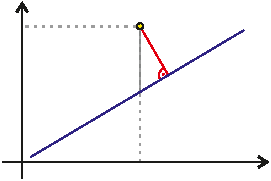
\includegraphics[width=7cm]{pictures/picture_2_F.pdf}};
    \draw [color=red](1.0,-0.45) node[anchor=north west] {$d$};
    \draw [color=red!20!black](1.35,1.00) node[anchor=north west] {Fisherova distribuce};
    \draw [color=black](-2.9,-1.25) node[anchor=north west] {nějaký text};
    \draw [color=black](-1,-1.25) node[anchor=north west] {$1$};
    \draw [color=black](0.75,-1.25) node[anchor=north west] {$a=bx$};
    \end{tikzpicture}
\end{center}

\begin{remark}
v literatuře se někdy $ x $ uvažují jako realizace náhodné veličiny ( ne vždy se $ x $ nastavuje předem, nebo je jasně dané (třeba pohlaví -- ???? (8 strana)) 
\end{remark}
Model má potom tvar
$$
 \E [ Y_{i} \vert X_{i} ] = \beta_{0} + \beta_{1} \quad  \D [ Y_{i} \vert X_{i} ] = \sigma^{2}
$$
pro většinu výsledků prezentovaných v této přednášce ale není podstatné, zde je $ x $ chápáno jako pevné nebo náhodné.
Důkazy většinou fungují s podmíněnými výrazy $ ( \E , \D , \dots )  $ při dané hodnotě $ x $ místo nepodmíněných.
Nicméně větší pozornost je třeba u odvození asymptotických rozdělení odhadů.

\subsection{Vlastnosti odhadů}
Vlastnosti odhadů $ \widehat{\beta}_{0} , \widehat{\beta}_{1} ,  s_{n}^{2} $.
\begin{theorem}
   Nechť $ \widehat{\beta}_{0} , \widehat{\beta}_{1} $ jsou $ \mathrm{LSE} $ odhady parametrů $ \beta_{0}, \beta_{1} $ v lineárním modelu 
   $$
   		Y_{i} = \beta_{0} + \beta_{1} x_{i} + e_{i} \quad i = 1 , \dots , n ,
   $$
   kde $ e_{i} $ jsou nezávislé náhodné veličiny (postačí i nekorelovanost) se stejným rozptylem $ \sigma^{2} $. Potom platí:
   \begin{enumerate}
  \item $ \E [ \widehat{\beta}_{0} ] = \beta_{0} \quad , \quad \E [ \widehat{\beta}_{1} ] = \beta_{1} $ , (nestranné odhady)
  \item $  \D [ \widehat{\beta}_{0} ] = \frac{\sigma^{2}}{S_{xx}}  \quad $ , kde $ \quad S_{xx} = \sumin (x_{i} - \oxnn )^{2} $
  \item $ \D [ \widehat{\beta}_{0} ] = \sigma^{2} \left( \frac{1}{n} + \frac{\oxnn ^{2}}{S_{xx}} \right) $
  \item Pokud navíc platí, že $ e_{i} \sim \NN ( 0 , \sigma^{2} ) \quad i = 1 , \dots , n \quad $ potom $ \quad \widehat{\beta}_{j} \sim \NN ( \beta_{j} , \D [ \widehat{\beta}_{j} ] ) \quad j = 0 , 1  $ 
\end{enumerate}
\end{theorem}
\begin{proofname}

   \begin{enumerate}
  \item upravíme $ \widehat{\beta}_{1} $
  		\begin{equation*}
  		\begin{aligned}
  		    \widehat{\beta}_{1} = \dfrac{\sum_{i=1}^{n} y_{i} x_{i} - n \overline{x}_{n} \overline{y}_{n}}{\sum_{i=1}^{n} x_{i}^{2} - n \overline{x}_{n}^{2}} = \frac{\sumin (x_i - \oxnn )(y_i - \oynn )}{\sumin (x_i - \oxnn )^{2}} = \\
  		    = \frac{1}{S_{xx}} \left( \sumin (x_i - \oxnn ) y_i - \oynn \sumin (x_i - \oxnn )  \right) =  \frac{1}{S_{xx}} \sumin (x_i - \oxnn ) y_i 
  		    \end{aligned}
  		\end{equation*}
  		potom má střední hodnota $ \widehat{\beta}_{1} $ tvar
  		\begin{equation*}
  		\begin{aligned}
  		    \E [ \widehat{\beta}_{1} ] = \E \left[ \frac{1}{S_{xx}} \sumin (x_i - \oxnn ) Y_i \right] = \frac{1}{S_{xx}} \sumin (x_i - \oxnn ) \E [ Y_i ] 
  		    = \frac{1}{S_{xx}} \sumin (x_i - \oxnn ) ( \beta_{0} + \beta_{1} x_i ) = \\ = \frac{\beta_{0}}{S_{xx}} \sumin (x_i - \oxnn ) + \frac{\beta_{1}}{S_{xx}} \sumin (x_i - \oxnn ) x_i = 0 + \frac{\beta_{1}}{S_{xx}} S_{xx} = \beta_{1}
  		    \end{aligned}
  		\end{equation*}
  		a střední hodnota pro $ \widehat{\beta}_{0} $ má tvar 
  		\begin{equation*}
  		\begin{aligned}
  		    \E [ \widehat{\beta}_{0} ] = \E [ \oyn - \widehat{\beta}_{1} \oxn ] = \E [ \oyn ] - \oxnn \E [ \widehat{\beta}_{1} ] = \dfrac{1}{n} \sumin \E [ Y_i ] - \oxnn \beta_1 = \beta_0 + \frac{\beta_1}{n} \sumin x_i - \oxnn \beta_1 = \beta_0
  		    \end{aligned}
  		\end{equation*}
  \item \begin{equation*}
  			\D [ \widehat{\beta}_{1} ] = \D \left[ \frac{1}{S_{xx}} \sumin (x_i - \oxnn ) Y_i \right] = \frac{1}{S_{xx} ^{2}} \sumin (x_i - \oxnn )^{2} \D [ Y_i ] = \frac{\sigma^{2} S_{xx}}{S_{xx}^{2}} = \frac{\sigma^{2}}{S_{xx}}
  		\end{equation*}
  \item  \begin{equation*}
  \begin{aligned}
  			\D [ \widehat{\beta}_{0} ] = \D [ \oyn - \widehat{\beta}_{1} \oxnn ] = \d [ \oyn ] + \oxnn ^{2} \D [ \widehat{\beta}_{1} ] - 2 \oxnn \text{cov}(\oyn , \widehat{\beta}_{1} ) = \\
  	= \frac{\sigma^{2}}{n} + \frac{\oxnn ^{2} \sigma^{2} }{S_{xx}} - 2 \oxnn \text{cov}( \oyn ,  \widehat{\beta}_{1} ) \\
\text{cov}( \oyn ,  \widehat{\beta}_{1} ) = \text{cov} \left( \oyn , \frac{1}{S_{xx}} \sumin ( x_i - \oxnn ) Y_i \right) = \frac{1}{S_{xx}} \sumin ( x_i - \oxnn ) \, \text{cov} ( \oyn , Y_i )  \\
\text{cov} ( \oyn , Y_i ) = \text{cov} ( \frac{1}{n} \sumjn Y_j , Y_i ) =  \frac{1}{n} \sumjn \text{cov} ( Y_j , Y_i ) = \frac{1}{n} \text{cov} ( Y_i , Y_i ) =  	\frac{1}{n} \D Y_i =  \frac{\sigma^{2}}{n}	\\
\Rightarrow  \text{cov}( \oyn ,  \widehat{\beta}_{1} ) = 0 = \frac{\sigma^{2}}{n S_{xx}} \sumin ( x_i - \oxnn )	
  			\end{aligned}
  		\end{equation*}
\end{enumerate}
\end{proofname}




\chapter{11-20}

\begin{theorem}
	Za předpokladu předchozí věty platí
	$$
		\E (s_n^2) = \sigma^2
	$$
	($s_n^2$ je nestranný odhad $\sigma^2$).
\end{theorem}


\begin{proof}
	$$
		\E(s_n^2)  = \frac{1}{n-2} \E \sum_{i=1}^{n} (Y_i - \hYi)^2 = \frac{1}{n-2} \underbrace{\sumin \E (Y_i - \hYi)^2}_{\text{ozn. } A}
	$$
	
	Protože $\E(\hYi)  = \E(\wbeta_0 + \wbeta_1 x_i) = \beta_0 + \beta_i x_i = \E Y_i$, platí, že:
	$$
	\E(Y_i - \hYi)^2   = \D(Y_i - \hYi) = \E (Y_i - \hYi)^2 - \underbrace{(\E(Y_i - \hYi)^2)}_{= 0}
	$$
	
	Dostáváme tak	
	\begin{align*}
		A & = \sum_{i=1}^{n} \D(Y_i - \hYi) = \sum_{i=1}^n [ \D(Y_i) + \D(\hYi) - 2 \Cov(Y_i, \hYi) ] =  \\
		& = n \sigma^2 + \sum_{i=1}^n \D(\hYi) - 2 \sum_{i=1}^n \Cov(Y_i, \hYi) \tag{$\#$}
	\end{align*}
	
	Rozepíšeme
	$$
		\D \hYi  = \D(\wbeta_o + \wbeta_1 x_i) = \D \wbeta_0 + x_i^2 \D \wbeta_1 + 2 x_i,
	$$
	kde
	$$
		\Cov(\wbeta_0, \wbeta_1) = \Cov(\hYn - \wbeta_1 \hxn, \wbeta_1) = \underbrace{\Cov(\hYn, \wbeta_1)}_{= 0 \text{ (viz. dříve)}} - \hxn \underbrace{\D(\wbeta_1)}_{\frac{\sigma^2}{s_{xx}}} = -\frac{\sigma^2 \hxn}{s_{xx}}
	$$
	a tedy
	\begin{align*}
		\D \hYi & = \sigma^2 \left[ \frac{1}{n} + \frac{\lxn^2}{s_{xx}} + x_i^2 \frac{1}{s_{xx}} - \frac{2 x_i \lxn}{s_{xx}} \right] = \sigma^2 \left[ \frac{1}{n} + \frac{(x_i - \lxn)^2}{s_{xx}}\right] \\
		\sum_{i=1}^n \D \hYi & = \sigma^2 + \frac{\sigma^2}{s_{xx}} \underbrace{\sum_{i=1}^n (x_i - \lxn)^2}_{ = s_{xx}} = 2\sigma^2
	\end{align*}
	
	Následně máme
	\begin{align*}
	\Cov(Y_i, \hYi) & = \Cov(Y_i, \wbeta_0 + \wbeta_1 x_0) = \Cov(Y_i, \wbeta_0) + x_i \Cov(Y_i, \wbeta_1) \\
	\Cov(Y_i, \wbeta_1) & = \frac{1}{s_{xx}} \sum_{j=1}^{n} (x_j - \lxn) \underbrace{\Cov(Y_i, Y_j)}_{= 0 \text{ pro } i \neq j} = \frac{\sigma^2(x_i - \lxn)}{s_{xx}} \\
	\Cov(Y_i, \wbeta_0) & = \Cov(Y_i, \bar{Y}_n - \lxn \wbeta_1) = \Cov(Y_i, \bar{Y}) - \lxn \Cov(Y_i, \wbeta_1) = \frac{\sigma^2}{n} - \frac{\lxn \sigma^2 (x_i - \lxn)}{s_{xx}} \\
	\end{align*}
	a tedy
	\begin{align*}
		\Cov(Y_i, \hYi) & = \frac{\sigma^2}{n} - \frac{\lxn \sigma^2 (x_i - \lxn)}{s_{xx}} + \frac{x_i \sigma^2 (x_i - \lxn)}{s_{xx}} = \frac{\sigma^2}{n} + \frac{\sigma^2}{s_{xx}}(x_i - \lxn)^2 \\
		\sum_{i=1}^n \Cov(Y_i, \hYi) & = \sigma^2 + \frac{\sigma^2}{s_{xx}} \sum_{i=1}^n (x_i - \lxn)^2 = 2 \sigma^2 \\
	\end{align*}
	Dosazením do ($\#$) dostaneme
	$$
		A  = n\sigma^2 + 2\sigma^2 - 4\sigma^2
	$$
	a celkem máme
	$$
		\E(s_n^2)  = \frac{1}{n-2} A = \sigma^2.
	$$
\end{proof}

\begin{corollary}
	Nechť platí předpoklady věty 1 a nechť $e_1, \dots, e_n~iid~\NN(0,\sigma^2)$. Potom platí:
	\begin{enumerate}[a)]
		\item $\frac{(n-2)s_n^2}{\sigma^2} \sim \chi(n-2)$
		\item $s_n^2$ je nezávislé na $\wbeta_0$ a $\wbeta_1$.
	\end{enumerate}
\end{corollary}

\begin{proof}
	Vyplyne z obecnějších tvrzení pro vícerozměrnou regresi.
\end{proof}

\begin{remark}
	Spočetli jsme
	$$
		\underbrace{\D(\wbeta_0)}_{\text{ozn. } \sigma^2(\wbeta_0)} = \sigma^2 \left[ \frac{1}{n} + \frac{\lxn^2}{s_{xx}} \right] \quad \text{a} \quad \underbrace{\D(\wbeta_1)}_{\text{ozn. } \sigma^2(\wbeta_1)} = \frac{\sigma^2}{s_{xx}}
	$$
	
	Nestranné odhady jsou:
	\begin{align*}
		\sigma^2(\wbeta_0) & = s_n^2 \sigma^2 \left[ \frac{1}{n} + \frac{\lxn^2}{s_{xx}} \right] = s_n^2 \delta_0 \\
		\sigma^2(\wbeta_1) & = \frac{s_n^2}{s_{xx}} = s_n^2 \delta_1,
	\end{align*}
	kde $\delta_0$ a $\delta_1$ jsou tzv. variance multiplication factors.
	
	Odhady směrodatné odchylky veličin $\wbeta_0$ a $\wbeta_1$ pak jsou
	$$
		\hat{\sigma}(\wbeta_0) = s_n \sqrt{\delta_0} \quad \text{a} \quad \hat{\sigma}(\wbeta_1) = s_n \sqrt{\delta_1},
	$$
	kterým se pak říká standardní chyby odhadů $\wbeta_0$ a $\wbeta_1$. Hrají zásadní roli při konstrukci IS a TH.
\end{remark}

\section{Gauss - Markov theorem}

\begin{itemize}
	\item Chyby normální $\Rightarrow$ LSE pro $\wbeta_0, \wbeta_1$ je MLE ... parametrů (eficientní odhad)
	\item Pokud nejsou chyby normální, jaké je opodstatnění použít LSE?
	
	Ukážeme, že LSE jsou BLUE (best linear unbiased estimators), tedy lineární nestranné odhady s minimálním rozptylem
	\item Je ale třeba poznamenat, že můžou existovat nelineární nebo vychýlené odhady parametrů $\beta_0, \beta_1$, které jsou eficientnější než LSE, pokud se rozdělení chyb liší výrazně od normálního (tím se zabývá robustní regresní analýza).
\end{itemize}

Uvažujme model
$$
	Y_i = \beta_0 + \beta_1 x_i + e_i, \quad i = 1, \dots, n \text{ (*)}
$$

\begin{define}
	Lineární odhad parametru $\beta$ je statistika tvaru
	$$
		\wbeta = \sumin c_i Y_i,
	$$
	kde $c_i$ jsou dané reálné konstanty a $i = 1, \dots, n$.
\end{define}

\begin{theorem}
	Nechť $e_1, \dots, e_n$ v modelu (*) jsou nekorelované a mají stejný rozptyl $\D(e_i) = \sigma^2, i = 1, \dots, n$. Potom LSE $\wbeta_j, j = 0,1$ je BLUE parametru $\beta_j$.
\end{theorem}

\newcommand{\pd}{\delta}

\begin{proof}
	Ukážeme pro $\beta_1$, pro $\beta_0$ je důkaz podobný.
	
	Nechť $\wbeta_1 = \sumin c_i Y_i$, pak
	
	$\D \wbeta_1 = \sumin c_i^2 \D Y_i = \sigma^2 \sumin c_i^2$
	
	Aby byl $\wbeta_1$ nestranný, musí platit $\E \wbeta_1 = \beta_1$, tedy
	
	$\E \wbeta_1 = \sumin c_i \E Y_i = \beta_0 \sumin c_i + \beta_1 \sumin c_i x_i \overset{!}{=} \beta_1$
	
	protože to musí platit pro lib. $\beta_0, \beta_1$, dostáváme
	$$
		\sumin c_i = 0 \quad \text{a} \quad \sumin c_i x_i = 1.
	$$
	
	Hledání lineárního, nestranného odhadu $\beta_1$ je tedy redukováno na minimalizaci $\sumin c_i^2$ za vazebných podmínek $\sumin c_i = 0 \quad \text{a} \quad \sumin c_i x_i = 1$.
	
	Lagrangeova funkce: $L = \sumin c_i^2 - 2 \lambda_1 (\sumin c_i) - 2 \lambda_2 (\sumin c_i x_i - 1)$.
	
	\begin{gather*}
		\frac{\partial L}{\partial c_i} = 2 c_i - 2 \lambda_1 - 2 \lambda_2 x_i = 0, \quad i = 1, \dots, n \\
		\frac{\partial L}{\partial \lambda_1} = -2 (\sumin c_i) = 0 \\
		\frac{\partial L}{\partial \lambda_2} = -2 (\sumin c_i x_i - 1) = 0
	\end{gather*}
	
	Sečteme prvních $n$ rovnic
	$$
		\underbrace{\sumin c_i}_{= 0} - n \lambda_1 - \lambda_2 \sumin x_i = 0 \Rightarrow n\lambda_1 + \lambda_2 \sumin x_i = 0 \Rightarrow \lambda_1 = - \lambda_2 \lxn
	$$
	
	Sečteme dále prvních $n$ rovnic vynásobených $x_i$:
	\begin{gather*}
		\sumin c_i x_i - \lambda_1 \sumin x_i - \lambda_2 \sumin x_i^2 = 0 \\
		\Rightarrow \lambda_1 \sumin x_i + \lambda_2 \sumin x_i^2 = 1 \\
		 -\lambda_2 \lxn \cdot n \lxn + \lambda_2 \sumin x_i^2 = 1 \\
		 \lambda_2 \left( \sumin x_i^2 - n \lxn^2 \right) = 1 \Rightarrow \lambda_2 = \frac{1}{s_{xx}} \quad \text{a} \quad \lambda_1 = - \frac{\lxn}{s_{xx}}
	\end{gather*}
	
	Dosadíme za $\lambda_1, \lambda_2$:
	$$
		c_i + \frac{\lxn}{s_{xx}} - \frac{x_i}{s_{xx}} = 0 \Rightarrow c_i = \frac{x_i - \lxn}{s_{xx}}
	$$
	a $\wbeta_1 = \frac{1}{s_{xx}} \sumin (x_i - \lxn) Y_i$, což je LSE.

\end{proof}

\begin{remark}
	Ukázali jsme pouze, že to je stacionární bod, že je tam i minimum ukážeme v obecnější větě ve vícerozměrné regresi.
\end{remark}

\section{IS pro $\beta_0, \beta_1$}

\begin{itemize}
	\item IS poskytují jistou "míru přesnosti" bodových odhadů
	\item pro jejich konstrukci potřebujeme znát rozdělení pravděpodobnosti bodového odhadu
	\item budeme tedy uvažovat normalitu chyb
	\item spočtené IS se ale často používají, i když rozdělení chyb není normální, jejich použití se zdůvodňuje tím, že LSE odhady par. $\beta$ jsou lineární funkcí $Y_i, i = 1, \dots, n$, což umožňuje aplikovat CLT a dostat asymptotickou normalitu odhadů $\wbeta_0, \wbeta_1$
\end{itemize}

Uvažujme model $Y_i = \beta_0 + \beta_1 x_i + e_i$, $e_i$ i.i.d $\NN(0,\sigma^2)$. Víme:
$$
	\wbeta_i \sim \NN(\beta_i, \sigma^2(\wbeta_i)), \quad \frac{(n-2)s_n^2}{\sigma^2} \sim \chi^2(n-1) \text{\; a nezávisí na \;} \wbeta_0, \wbeta_1.
$$

\begin{remark}
	$$
		X \sim \NN(0,1), Y \sim \chi^2(n), X, Y \text{ nezávislé } \Rightarrow \frac{X}{\sqrt{Y/n}} \sim t(n)
	$$
\end{remark}

Tedy
$$
	T_i = \frac{\frac{\wbeta_i - \beta_i}{\sigma(\wbeta_i)}}{\frac{s_n}{\sigma}} = \frac{\wbeta_i - \beta_i}{\hat{\sigma}}(\wbeta_i) \sim t(n-2, i = 0,1)
$$
neboť $\sigma(\wbeta_i) = \sigma \sqrt{\delta_i}$ a $\hat{\sigma}(\wbeta_i) = s_n \sqrt{\delta_i}$.

Tzn. $P \left[ -t_{1-\alpha/2}(n-2) \leq \frac{\wbeta_i - \beta_i}{\hat{\sigma}}(\wbeta_i) \leq t_{1-\alpha/2}(n-2) \right]$ a vyjádřením $\beta_i$ dostaneme
$$
	P \left[ \wbeta_i - t_{1-\alpha/2}(n-2) \hat{\sigma}(\wbeta_i) \leq \beta_i \leq  \wbeta_i + t_{1-\alpha/2}(n-2) \hat{\sigma}(\wbeta_i) \right] = 1 - \alpha
$$
a tedy $(\wbeta_i \pm t_{1-\alpha/2}(n-2) \hat{\sigma}(\wbeta_i))$ je $100(1-\alpha)\%$ IS pro $\beta_i, i = 0,1$.

Dosazením za $\hat{\sigma}(\wbeta_i)$ dostaneme

\begin{itemize}
	\item $100(1-\alpha)\%$ IS pro $\beta_0$: $\wbeta_0 \pm t_{1-\alpha/2}(n-2) \cdot s_n \sqrt{\frac{1}{n} + \frac{\lxn^2}{s_{xx}}}$
	\item $100(1-\alpha)\%$ IS pro $\beta_1$: $\wbeta_1 \pm t_{1-\alpha/2}(n-2) \cdot s_n \frac{1}{\sqrt{s_{xx}}}$
\end{itemize}

\begin{remark}
	Z tvarů IS lze pozorovat, že IS pro $\beta_0$ bude ve většině praktických případů širší než IS pro $\beta_1$, tzn. směrnice je obecně odhadnuta s větší přesností než absolutní člen (intercept).
\end{remark}


\begin{remark}
	Někdy se konstruují simultánní IS pro oba parametry. (Obr?) Zmíníme podrobněji u vícerozměrné regrese.
\end{remark}


\section{TH pro $\beta_0, \beta_1$}

Chtěli bychom ověřit platnost předpokladu lineárního vztahu mezi $x$ a $y$.

Předpokládejme nyní, že model je lineární a že $x$ je jediná dostupná vysvětlující proměnná. Otázoku je, zda je $x$ užitečná ve vysvětlení variability v $y$, chceme tedy rozhodnout mezi dvěma modely:
$$
	Y_i = \beta_0 + e_i \quad \text{a} \quad Y_i = \beta_0 + \beta_1 x_i + e_i
$$
tzn. otestovat hypotézu $\hypothesis{\beta_1 = 0}{}\beta_1 \neq 0$.

Pokud nezamítneme $H_0$, závěr bude, že $x$ nevysvětluje nic z variability $y$ a není v modelu významné. Pokud zamítneme $H_0$, znamená to, že $x$ je významné.

\begin{remark}
	Tyto závěry jsou správné pouze za předpokladu, že model je lineární!
	\begin{itemize}
		\item nezamítnutí $H_0$ nemusí znamenat, že $x$ není užitečná, může to pouze indikovat, že vztah mezi $y$ a $x$ není lineární
		\item zamítnutí $H_0$ naopak ří, že existuje lineární trend mezi $x$ a $y$, ale mohou tam být i jiné typy závislosti
	\end{itemize}
\end{remark}

Pro konstrukci testů využijeme odvozené IS.

\begin{remark}
	Opakování: $\hypothesis{\theta = \theta_0}{\theta \neq \theta_0} \Rightarrow (\underline{\theta}, \bar{\theta})$ je $100(1-\alpha)\%$ IS pro $\theta$. Pak $W = \{ x | \theta_0 \notin (\underline{\theta}, \bar{\theta}) \}$ je kritický obor test na hladině $\alpha$.
\end{remark}

$H_0: \beta_1 = 0$ zamítneme, pokud $0 \notin \left( \wbeta_1 \pm t_{1-\alpha/2}(n-2) \cdot  \frac{s_n}{\sqrt{s_{xx}}} \right)$, tzn.
\begin{gather*}
	\text{buď } \wbeta_1 + t_{1-\alpha/2}(n-2) \cdot  \frac{s_n}{\sqrt{s_{xx}}} < 0 \iff  \wbeta_1 \frac{\sqrt{s_{xx}}}{s_n} < - t_{1-\alpha/2}(n-2) \\
	\text{nebo } \wbeta_1 - t_{1-\alpha/2}(n-2) \cdot  \frac{s_n}{\sqrt{s_{xx}}} > 0 \iff \wbeta_1 \frac{\sqrt{s_{xx}}}{s_n} > t_{1-\alpha/2}(n-2)
\end{gather*}
A zapsáno dohromady
$$
	|T_n| = |\wbeta_1| \frac{\sqrt{s_{xx}}}{s_n} > t_{1-\alpha/2}(n-2).
$$

\begin{remark}
	Intuitivní interpretace: $|T_n| = |\wbeta_1| \frac{\sqrt{s_{xx}}}{s_n} = \frac{|\wbeta_1|}{\hat{\sigma}(\wbeta_1)}$ je převrácená hodnota relativní chyby.
	
	Pokud je $\beta_1$ dobře odhadnuto, očekáváme malý rozptyl $\hat{\sigma}(\wbeta_1)$, tedy $T$ bude velké.
	
	t-test tedy říká, že zamítneme $H_0$, pokud je relativní chyba odhadu malá.
\end{remark}
\chapter{21-30}
\begin{remark}
	Někdy dopředu známe kandidáta $b_1$ jako hodnotu parametru $\beta_1$ a~chtěli bychom testovat 
	$\hypothesis{\beta_1=b_1}{\beta_1\neq b_1}$. Test bude zamítnut $H_0$, pokud 
	$$ \abs{\beta_1-b_1}\cdot \frac{\sqrt{S_{xx}}}{s_n}> t_{1-\frac{\alpha}{2}}(n-2). $$
\end{remark}
\subsection{Test významnosti interceptu}
Otázka je, zda přímka prochází počátkem $(0,0)$, tedy $\hypothesis{\beta_0=0}{\beta_0\neq0}$. Nezamítnutí $H_0$ znamená, že jednodušší model $y=\beta_1 x+e$ lépe popisuje datta, než $y=\beta_0+\beta_1 x+e$. $H_0$ potom zamítneme, pokud
$$ T_n=\frac{|\widehat{\beta}_0|}{\widehat{\sigma}(\widehat{\beta}_0)}=|\widehat{\beta}_0|\frac{1}{s_n\sqrt{\frac{1}{n}+\frac{\overline{x}^2}{S_{xx}}}}>t_{1-\frac{\alpha}{2}}(n-2). $$

\subsection{ANOVA přístup pro~testování}
Odvodili jsme $t$-test významnosti koeficientů a~nyní odvodíme ekvivalentní $F$-test, který může být zobecněn na~test celkové významnosti vícerozměrného regresního modelu (testy významnosti jednotlivých koeficientů mohou být totiž zavádějící). 

Myšlenkou metody (analýza rozptylu ANOVA) je určit, kolik variability v~pozorováních $(y_1,y_2,...,y_n)$ je "vysvětleno" regresním modelem (přímkou). Míru variability v~datech pak spočítáme jako podíl součtu sum od~regrese a~celkového počtu čtverců, tedy
$$ \SST=\sum_{i=1}^{n}(y_i-\overline{y}_n)^2, $$
pokud regresní přímka $y=\widehat{\beta}_0+\widehat{\beta}_1 x$ dobře prokládá data, tedy $\widehat{y}_i\approx y_i$. Dále bude platit, že 
$$ \sumin (\hyi-\lhyn)^2\approx\sumin (y_i-\lyn)^2. $$
Ukážeme, že $\lhy=\lyn$ a~tak 
$$ \sumin(\hyi-\lhyn)^2=\sumin (\hyi-\lyn)^2=\SSR $$ regresi sum ob squares, regresní součet čtverců. Podíl
$$ \RMR^2=\frac{\SSR}{\SST}=\frac{\sumin (\hyi-\lyn)^2}{\sumin (y_i-\lyn)^2}$$ tak vyjadřuje variabilitu v~$(y_1,...,y_n)$ vysvětlené regresním modelem. 

$\RMR^2$ - \textit{koeficient determinace (coefficient of determination)} (pro každý model by měl mít hodnotu $\RMR^2\approx 1$). Ukážeme, že $\RMR^2$ je kvadrát výběrového korelačního koeficientu mezi~$\textbf{x}$ a~$\textbf{y}$, což dává statistice $\RMR^2$ význam míry "dobré shody". 

Pokud bychom znali rozdělení pravděpodobnostní statistiky $\RMR^2$, nabízí se~její použití pro~test $H_0:~\beta_1=0$, kterou bychom zamítli, pokud bude $\RMR^2\approx1$. Protože každá monotonní funkce $\RMR^2$ vede na~ekvivalentní test, budeme uvažovat statistiku $$ \mathrm{F}=\frac{(n-2)\RMR}{1-\RMR^2}. $$

\begin{lemma}\label{lemma_k_vete}
	Nechť $\widehat{e}_i=y_i-\hyi$ značí rezidua, kde $\hyi=\wbeta_0+\wbeta_1 x_i$ a~$ \wbeta_0,\wbeta_1$ jsou LSE. Potom \begin{enumerate}
		\item $\sumin\widehat{e}_i=0$,
		\item $\lhyn=\lyn$,
		\item $\sumin \widehat{e}_i\hyi=0$.
	\end{enumerate}
\begin{proof}
	\begin{enumerate}
		\item Z~rovnice $\frac{\partial S}{\partial\beta_0}=0$ dostaneme $$ 0=\sumin (y_i-\wbeta_0-\wbeta_1 x_i)=\sumin(y_i-\hyi)=\sumin \widehat{e}_i.$$
		\item Z~bodu 1) plyne, že $\sumin\hyi=\sumin y_i$, podělením $n$ dostaneme dokazované tvrzení.
		\item Z~rovnice $\frac{\partial S}{\partial\beta_1}=0$ dostaneme $$0=\sumin(y_i-\wbeta_0-\wbeta_1 x_i)x_i=\sumin \hei x_i$$ a~tedy $$ \sumin \hei\hyi=\sumin \hei (\wbeta_0+\wbeta_1 x_i)=\sumin\hei\wbeta_0+\sumin x_i \hei\wbeta_1=\wbeta_0\underbrace{\sumin \hei}_{=0}+\wbeta_1\underbrace{\sumin x_i\hei}_{=0}=0.$$
	\end{enumerate}
\end{proof}
\end{lemma}
\begin{theorem}
	Předpokládejme, že $\SST\neq 0$. Potom platí\begin{enumerate}
		\item $0\leq \RMR^2\leq1$,
		\item $\RMR^2=1-\frac{\SSE}{\SST}$, kde $\SSE=\sumin(y_i-\hyi)^2$ jako reziduální součet čtverců,
		\item $\RMR^2=1~\Leftrightarrow~(\forall i~\in\hat{n})(\hyi=y_i)$ (všechna data leží na~přímce),
		\item pokud označíme $\textbf{x}=(x_1,...,x_n)$ a~$\textbf{y}=(y_1,...,y_n)$, potom $\RMR^2=\rho^2(\textbf{x},\textbf{y})$, kde $$\rho(\textbf{x},\textbf{y})=\frac{\Big(\sumin(x_i-\overline{x}_n)(y_i-\lyn)\Big)^2}{S_{xx}S_{yy}}$$ je druhá mocnina výběrového korelačního koeficientu vektorů $\textbf{x},\textbf{y}$,
		\item $\mathrm{F}=\frac{\SSR}{s_n^2}=\mathrm{T}^2$,
		\item pokud jsou chyby $e_1,...,e_n~iid~\NN(0,\sigma^2)$ a~$\beta_1=0$ (platí $H_0:~\beta_1=0$) v~modelu, potom  $\mathrm{F}\sim\mathrm{F}(1,n-2)$.
	\end{enumerate}
\begin{proof}
	Důkaz věty bude založen na~rozkladu
	$$ \sumin (y_i-\lyn)^2=\sumin(\hyi-\ly)^2 + \sumin (y_i-\hyi)^2 $$ neboli $\SST=\SSR+\SSE$. Z~lemmatu \ref{lemma_k_vete} vyplývá, že 
	\[
	\begin{split}
	\SST&=\sumin (y_i-\lyn)^2=\sumin\big[ (y_i-\hyi)+(\hyi-\lyn) \big]^2=\\&=\sumin(y_i-\hyi)^2+\sumin(\hyi-\lyn)^2+2\sumin(y_i-\hyi)(\hyi-\lyn)=\SSE+\SSR+0 ,
	\end{split}
	\]
	neboť $$ \sumin(\underbrace{(y_i-\hyi)}_{=\hei}(\hyi-\lyn))=\underbrace{\sumin\hei\hyi}_{=0}-\lyn\underbrace{\sumin\hei}_{=0}=0.$$
	Z toho potom dokazujeme jednotlivé body věty. \begin{enumerate}
		\item Protože $\SST=\SSE+\SSR$, pak $0\leq \RMR^2=\frac{\SSR}{\SST}\leq \frac{\SST}{\SST}=1$.
		\item $\SSR=\SST-\SSE~\Rightarrow~\RMR^2=\frac{\SST-\SSE}{\SST}=1-\frac{\SSE}{\SST}$.
		\item Z~bodu 2 plyne, že $\RMR^2=1~\Leftrightarrow~\SSE=0$ a~$\SSE=\sumin(y_i-\hyi)^2=0~\Leftrightarrow~y_i=\hyi ~\forall i~\in\hat{n}$.
		\item  $\hyi=\underbrace{\wbeta_0}_{=\lyn=\wbeta_1 x_n} + \wbeta_1 x_i=\lyn-\wbeta_1(\overline{x}_n-x_i)$. Proto pak $$ \SSR=\sumin(\hyi-\hyn)^2+\wbeta_1^2\sumin(x_i-\overline{x}_n)^2=\wbeta_1^2 S_{xx},$$ a~protože $\wbeta_1=\frac{1}{S_{xx}}\sumin(x_i-\overline{x}_n)(y_i-\lyn)$, dostaneme 
		$$ \rho^2(\textbf{x},\textbf{y})=\frac{\Big[\sumin(x_i-\overline{x}_n)(y_i-\lyn)\Big]^2}{S_{xx}S_{yy}}=\frac{\wbeta_1^2 S_{xx}}{S_{yy}}=\frac{\SSR}{\SST}=\RMR^2, $$ neboť $S_{yy}=\sumin(y_i-\lyn)^2=\SST$.
		\item Z~definice $\mathrm{F}$ plyne, že 
		$$ \mathrm{F}=\frac{(n-2)\RMR^2}{1-\RMR^2}=\frac{(n-2)\frac{\SSR}{\SST}}{\frac{\SSE}{\SST}}=\frac{\SSR}{\frac{\SSE}{n-2}}=\frac{\SSR}{s_n^2}. $$ Protože $T_n=\wbeta_1\frac{\sqrt{S_{xx}}}{s_n}$, pak $$ \mathrm{T}^2=\frac{\wbeta_1^2 S_{xx}}{s_n^2}=\frac{\SSR}{s_n^2}=\mathrm{F}. $$
		\item $T\sim t(n-2)~\Rightarrow~\mathrm{F}=\mathrm{T}^2\sim\mathrm{F}(1,n-2)$.
		
	\end{enumerate}
\end{proof}
\end{theorem}
\begin{remark}
\begin{enumerate}
	\item 	Z bodů 5 a~6 vyplývá, že použití libovolné statistiky $T_n,\RMR^2$ nebo $\mathrm{F}$ vede na~ekvivalentní test významnosti regrese.
	\item $\RMR^2$ poskytuje hrubou představu o~kvalitě modelu, čím je blíže $1$, tím lépe přímka prokládá data (nicméně je třeba jisté obezřetnosti, jak uvidíme později).
	\item $\mathrm{F}$ lze chápat jako statistiku pro~test významnosti velkých hodnot $\RMR^2$.
\end{enumerate}
\end{remark}
Výsledky se~většinou uvádí v~tabulce ANOVA:
\begin{table}[h]\label{ANOVA_table}
	\begin{tabular}{|lllll|}
	\hline
	Source & df & SS & MS & F\\
	\hline
	Regression & 1 & SSR & MSR=SSR & $\frac{\mathrm{MSR}}{\mathrm{MSE}}$ \\
	Residual & $n-2$ & SSE & $\mathrm{MSE}=\frac{\mathrm{SSE}}{n-2}=s_n^2$ & \\
	Total & $n-1$ & SST & & \\ \hline
\end{tabular}
\end{table}

$$\RMR^2=\frac{\SSR}{\SST}$$
Kde \textbf{source} je zdroj součtu čtverců, \textbf{df} počet stupňů volnosti příslušný danému součtu čtverců, \textbf{SS} počet čtverců a~\textbf{MS} $(\mathrm{MS}=\frac{\mathrm{SS}}{\mathrm{df}})$ "mean squares". 
\begin{remark}
	$H_0:~\beta_1=0$ je zamítnul, pokud $\mathrm{F}>\mathrm{F}_{1-\alpha}(1,n-2)$. V~tomto jednorozměrném případě je to ekvivalentní $t$-testu, neboť $\mathrm{F}=\mathrm{T}^2$.
\end{remark} 
\begin{theorem}
	Mějme $e_1,...,e_n~iid~\NN(0,\sigma^2)$. Za~platnosti $H_0:~\beta_1=0$ je splněno, že
	$$ \frac{\SSR}{\sigma^2}\sim\chi^2(1),\qquad\frac{\SSE}{\sigma^2}\sim\chi^2(n-2),\qquad\frac{\SST}{\sigma^2}\sim\chi^2(n-1). $$
\end{theorem}
\begin{remark}
	Proto v~tabulce ANOVA \ref{ANOVA_table} uvádí df po~řadě $1,n-2,n-1$. Používají se~však i~v případě jiného rozdělení chyb. Představit si je lze takto:\begin{enumerate}
		\item $\SSE=\sumin\hei^2$, na~$n$-rezidní $\he_1,...,\he_n$ máme 2 podmínky $\sumin\hei=0$ a~$\sumin x_i\hei=0$. Z~toho vyplývá, že mají $n-2$ stupňů volnosti.
		\item $\SST=\sumin(y_i-\lyn)^2$... $y_i-\lyn$ musí splňovat $\sumin(y_i-\lyn)=0$, a~proto má $n-1$ stupňů volnosti.
		\item $\SSR=\SST-\SSE$, a~počet stupňůů volnosti je roven $(n-1)-(n-2)=1$.
	\end{enumerate} 
\begin{proof}
	V důkazu věty ?? jsme ukázali, že $\SSR=\wbeta_1^2 S_{xx}$, takže $\frac{\SSR}{\sigma^2}=\Big( \frac{\wbeta_1\sqrt{S_{xx}}}{\sigma} \Big)^2$, víme, že $\wbeta_1\sim\NN\big(\beta_1,\frac{\sigma^2}{S_{xx}}\big)$ a~tedy $(\wbeta_1-\beta_1)\frac{S_{xx}}{\sigma}\sim\NN(0,1)$. Pro~$\beta_1=0$ tedy $$\wbeta_1\frac{\sqrt{S_{xx}}}{\sigma}\sim\NN(0,1)~\Rightarrow~\frac{\SSR}{\sigma^2}\sim\chi^2(1).$$
	Zároveň také $\frac{\SSE}{\sigma^2}=\frac{(n-2)s_n^2}{\sigma^2}\sim\chi^2(n-2)$ (viz dříve) a~nezávisí na~$\wbeta_1$. Z~toho vyplývá, že $\frac{\SSR}{\sigma^2}$ a~$\frac{\SSE}{\sigma^2}$ jsou nezávislé. Dále platí, že 
	$$ \frac{\SST}{\sigma^2}=\frac{\SSR}{\sigma^2}+\frac{\SSE}{\sigma^2}~\Rightarrow~\frac{\SST}{\sigma^2}\sim\chi^2(n-1).$$
\end{proof}
\end{remark}
\begin{remark}
	$\RMR^2$ statistika - pozor na~zjednodušení kvality modelu. \begin{enumerate}
		\item Nízké hodnoty $\RMR^2$ nemusí znamenat, že regresní model není významný. V~datech jen může být velké množství nevysvětlitelné náhodné variability. Například opakování hodnoty regresoru $x$ snižují hodnotu $\RMR^2$ oproti~modelům s~různými $x$.
		\item Velké hodnoty $\RMR^2$ mohou být způsobeny velkým měřítkem dat ($S_{xx}$ je velká). Platí totiž, že 
		$$ \E(\RMR^2)\approx\frac{\beta_1^2 S_{xx}}{\beta_1^2 S_{xx}+\sigma^2},$$ což je rostoucí funkce $S_{xx}$.
		
		Velký rozptyl $(x_1,...,x_n)$ může mít za~následek velké $\RMR^2$ a~přitom nic neříká o~kvalitě modelu.
		
		$\E(\RMR^2)$ je také rostoucí funkcí $\beta_1^2$. Modely s~$velkou$ směrnicí tedy budou mít obecně větší $yRMR^2$, než modely s~"malou" směrnicí. 
	\end{enumerate}
\end{remark}

Při hodnocení kvality modelu potřebujeme více kritérií. Mezi~ně patří například\begin{enumerate}
	\item "velké" $\RMR^2$,
	\item "velké" $\mathrm{F}$ nebo $|\mathrm{T}|$ hodnoty,
	\item "malé" hodnoty $s_n^2$ vzhledem k~$\lyn$.
\end{enumerate}
Další kritéria budeme probírat později.
\begin{example}
	Velká hodnota $\RMR^2$ indikuje přibližně lineární vztah mezi~$x$ a~$y$, ale vysoký stupeň korelace nemusí znamenat příčinný vztah.
	data: 1924-1937
	
	$y_i$ - počet mentálních onemocnění na~$100000$ obyvatel Anglie.\\
	$x_i$ - počet rádií v~populaci.\\
	model - $y_i=\beta_0+\beta_1 x_i+e_i$.
	$$ \wbeta_0=4.5822,\qquad\wbeta_1=2.2042,\qquad\RMR^2=0.984,$$
	tzv. velmi významný lineární vztah mezi~$x$ a~$y$. Závěr by mohl být, že rádia způsobují mentální onemocnění. I~když by to mohla být pravda, nabízí se~věrohodnější vysvětlení, a~to takové, že $x$ i~$y$ rostou lineárně s~časem, tzn. $y$ roste lineárně s~$x$. 
	
	Rádia byla s~časem dostupnější, lepší diagnostické procedury umožňovaly identifikovat více lidí s~mentálními problémy.
\end{example}
% pages 31-35
\begin{remark}
 korelace VS příčinnost
 
 \begin{itemize}
  \item \textbf{Příčinná spojitost} - i když je příčinná spojitost mezi $ x $ a $ y $ korelace samotná nám neřekne, zda $ x $ ovlivňuje $ y $ nebo naopak.
  \item \textbf{Skrytá příčinnost} - skrytá veličina $ z $ ovlivňuje $ x $ i $ y $, což způsobuje jejich korelovanost.
  \item \textbf{Confounding factor} - skryté proměnné $ z $ i $ x $ ovlivňují $ y $, výsledek tedy závisí i na $ z $.
  \item \textbf{Coincidence} - korelace je náhodná.
\end{itemize}
\end{remark}

\section{Regrese skrz počátek}
Existují případy, kdy přípustný model vyžaduje $ \beta_0 = 0 $, tj. 
$$
 Y_i = \beta_1 x_i + e_i \, , \quad \text{kde} \quad i = 1,\dots,n
$$

\begin{example}
 \begin{itemize}
  \item Je to předem známo na základě nějakých fyzikálních úvah 
  $$
 \E [Y_0] = \beta_0 = 0
$$
		potom nemá smysl odhadnout $ \beta_0 $, protože to obecně sníží přesnost odhadu $ \sigma^{2} $ a tedy i $ \beta_1 $
  \item Na začátek předpokládáme, že $ \beta_0 \neq 0 $ a t-test nezamítne hypotézu $ \text{H}_0 \, : \, \beta_0 = 0 $, potom $ \beta_0 $ může být z modelu odstraněn.
\end{itemize}
\end{example}

\begin{remark}
V praktických situacích si často nemůžeme být jisti, že model platí i blízko počátku. Část statistiků trvá na přítomnosti interceptu v modelu, i když je nevýznamný.

Položit $ \beta_0 $ apriorně, může nýt chybné i když $ \E [ Y_0 ] = 0 $. Pokud totiž nevíme jistě, že model je lineární na okolí 0, volba $ \beta_0 = 0 $ může vést k vychýleným odhadům $ \beta_1 $, pokud jsou nezávislé proměnné daleko od $ x = 0 $.
\end{remark}

----------------PICTURE----------------------

\subsection{Odhady a testy v případě $ \beta_0 = 0 $}
LSE parametru $ \beta_1 $ dostaneme minimalizací $ S = \sumin ( y_i - \beta_1 x_i )^{2}  $ ve tvaru: 
$$ 
 \widehat{\beta}_{1} = \dfrac{\sumin  y_i  x_i }{\sumin x_i^{2}},
$$
pokud $ e_1,\dots , e_n  $ i.i.d. $ N(0,\sigma^{2}) $, potom $ \E [ \widehat{\beta}_{1} ] = \beta_1 $ a $ \D [ \widehat{\beta}_{1}  ] = \frac{\sigma^{2}}{\sumin x_i^{2}} $.
Takže $  \widehat{\beta}_{1} \sim N(\beta_1 , \frac{\sigma^{2}}{\sumin x_i^{2}}) $
a $ s_n^{2} = \dfrac{\sumin (y_i -  \widehat{y}_i)^{2}}{n-1} = \dfrac{\SSE}{n-1} $ je nestranný odhad $ \sigma^{2} $.
Dále $ \frac{\SSE}{\sigma^{2}} \sim \chi^{2}(n-1) $ a nezávisí na $ \widehat{\beta}_{1} $.
$ \text{H}_0 \, : \, \beta_1 = 0 $ lze otestovat za pomoci statistiky:
$$ 
  T = \dfrac{\widehat{\beta}_{1}}{\dfrac{s_n}{\sqrt{\sum x_i^{2}}}} \sim \text{t}(n-1)
$$

$ 100(1-\alpha) \% $ IS pro $ \beta_1 $ je $ (\widehat{\beta}_{1} \pm \text{t}_{1 - \dfrac{\alpha}{2}}(n-1)\dfrac{s_n}{\sqrt{\sum x_i^{2}}}) $
\begin{itemize}
  \item Zatím je vše podobné jako pro případ $ \beta_1 \neq 0 $.
  \item Rozdíl je ale v tabulce ANOVA a v míře dobré shody, problém je, že neplatí rozklad $ \SST = SSR + SSE $ neboť součet reziduí $ \sumin (y_i - \widehat{y}) $ nemusí být 0 a tedy $ \overline{\widehat{y}}_n \neq \overline{y}_n $.
  Odvodíme nový rozklad, který platí v obou případech, dokážeme ho ale jen pro $ \beta_0 = 0 $
\end{itemize}

\begin{theorem}
V modelu s $ \beta_0 = 0 $ platí
$$ 
 \sumin y_i^{2} = \sumin \widehat{y}_i^{2} + \sumin ( y_i - \widehat{y}_i )^{2}
$$
\end{theorem}

\begin{proof}
$$ 
 \sumin y_i^{2} = \sumin (y_i - \widehat{y}_i + \widehat{y}_i )^{2} = \sumin ( y_i - \widehat{y}_i )^{2} + \sumin \widehat{y}_i^{2} + 2 \sumin ( y_i - \widehat{y}_i ) \widehat{y}_i 
 $$
 $$
 \text{z rovnice}  \quad  \dfrac{\d S}{\d \beta_1} = 0  \quad  \text{dostaneme}  \quad \sumin ( y_i - \widehat{\beta}_1 x_i) x_i = 0
$$
 $$
 \sumin ( y_i - \widehat{y}_i ) \widehat{y}_i  = 0  \quad \text{Q. E. D.}
$$
\end{proof}
Pokud vezmeme $ \sum y_i^{2} $ jako míru variability v datech, analogie $ \text{R}^{2} $ statistiky bude

$$ 
  \text{R}^{2} = \dfrac{\sumin \widehat{y}_i^{2}}{\sumin y_i^{2}} \quad \Leftrightarrow \quad
  1 - \text{R}^{2} = \dfrac{\sumin y_i^{2} - \sumin \widehat{y}_i^{2}}{\sumin y_i^{2}} = \dfrac{\sumin \widehat{e}_i^{2}}{\sumin y_i^{2} }
$$
=definujeme $ \FF = \dfrac{(n-1) \text{R}^{2}}{1 - \text{R}^{2}} $ potom 
$$ 
  \FF = \dfrac{\sumin \widehat{y}_i^{2} }{\frac{1}{n-1} \sumin ( y_i - \widehat{y}_i )^{2} } = \dfrac{\widehat{\beta}_{1} \sumin x_i^{2} }{ s_n^{2}}= \text{T}^{2}
$$

vztah mezi $ \text{R}^{2}, \FF \text{ a T}^{2} $ je tedy stejný jako pro $ \beta_0 \neq 0 $.

\begin{remark}
  Tato definice $ \text{R}^{2} $ se ale v praxi moc nepoužívá, protože neumožňuje přímé srovnání modelů bez a s interceptem.
\end{remark}

\noindent\begin{minipage}{.5\linewidth}
$$
  \beta_0 = 0 \quad : \quad \text{R}^{2} = 1 - \dfrac{\SSE}{\sumin y_i^{2}}
$$
\end{minipage}%
\begin{minipage}{.5\linewidth}
$$
  \beta_0 \neq 0 \quad : \quad \text{R}^{2} = 1 - \dfrac{\SSE}{\sumin (y_i - \oynn)^{2}}
$$
\end{minipage}

obecně ale $ \sumin (y_i - \oynn)^{2} < \sumin y_i^{2} $, $ \text{R}^{2} $ v modelu s $ \beta_0 = 0 $ tedy bude větší než $ \text{R}^{2} $ modelu s $ \beta_0 \neq 0 $ i když jsou jejich $ \SSE $ srovnatelné.

\begin{itemize}
  \item Definice vhodné $ \text{R}^{2} $ pro $ \beta_0 = 0 $ vyvolává jistou kontroverzi a existuje několik verzí.
  \item Možná volba je $ \text{R}^{2} = ( \rho (y_I, \overline{y}_{I}  ))^{2} $, kde $ \overline{y}_{I} = ( \overline{y}_{1},\dots ,\overline{y}_{n}) $ protože tato vlastnost platí i pro případ $ \beta_0 = 0 $.
  \item Další možnost je srovnat modely pomocí hodnot $ s_n^{2} $. (preferuje se model s nejnižší hodnotou $ s_n^{2} $)
\end{itemize}
\begin{table}[h]
	\begin{tabular}{lllll}
		Source & df & SS & MS & F \\
		\hline
		Regression & $1$ & SSR$=\sumin \hyi^{2}$ & MSR$=\frac{\SSR}{1}$ & $\frac{\SSR}{s_n^{2}}$ \\
		Residual & $n-1$ & SSE$=\sumin(y_i=\hyi)^{2}$ & MSE$=\frac{\SSE}{n-1}$ &  \\
		Total & $n$ & $\SST=\sumin y_i^{2}$ &  &  \\
		\hline
		&  & $\RMR^{2}=\rho^{2}(\textbf{y},\widehat{\textbf{y}})$ &  &  \\
	\end{tabular}
\caption{Tabulka ANOVA pro~$\beta_0=0$.}
\end{table}

\subsection*{Predikce}
Jakmile máme model, často bývá cílem odhadnout hodnoty veličiny $Y_0$ pro~nové $x_0$, které není v~původních datech. Budeme uvažovat dva typy predikce:\begin{enumerate}
	\item predikce střední hodnoty $\mu_0=\EE{Y_0}$ v~bodě $x_0$,
	\item predikce hodnoty nového pozorování $Y_0$ v~bodě $x_0$.
\end{enumerate}
Pro oba typy použijeme bodový odhad 
$$ \widehat{Y}_0=\wbeta_0+\wbeta_1 x_0.$$
Intervalové odhady se~ale budou lišit.

\subsection{Ad 1}
	Protože je $\mu_0=\beta_0+\beta_1 x_0$ vlastně parametr, lze pro~něj odvodit IS (za předpokladu normality chyb). 
	
	Spočteme tedy $\D(\widehat{Y}_0)$. Dosazením odhadů $\wbeta_0$ a~$\wbeta_1$ dostaneme $\widehat{Y}_0=\overline{y}+\wbeta_1(x_0-\overline{x})$ a
	$$ \D\widehat{Y}_0=\D(\overline{Y})+(x_0-\overline{x})^2\D(\wbeta_1)+2(x_0-\overline{x})\underbrace{\Cov(\overline{Y},\wbeta_1)}_{=0}=\frac{\sigma^2}{n}+\frac{\sigma^2(x_0-\overline{x})^2}{S_{xx}}=\sigma^2\Big[ \frac{1}{n}+\frac{(x_0-\overline{x})^2}{S_{xx}} \Big].$$
	
	Nahrazením $\sigma^2$ statistika $s_n^2$ dostaneme odhad $\D(\widehat{Y}_0)$ ve~tvaru 
	$$ \widehat{\sigma}^2(\overline{Y}_0)=s_n^2\Big[ \frac{1}{n}+\frac{(x_0-\lx)^2}{\Sxx} \Big].$$
	$\wsigma(\hY_0)$ se~obvykle nazývá \textbf{standardní chyba predikce v~bodě $x_0$}. Jsou-li $e_1,...,e_m~iid\N(0,\sigma^2)$, platí, že 
	$$ \hY_0\sim\N\Big( \mu_0,\underbrace{\sigma^2\Big[ \frac{(x_0-\lx)^2}{\Sxx} \Big]}_{\sigma^2(\hY_0)} \Big) $$ a~tedy 
	$$ \frac{\hY_0-\mu_0}{\sigma(\hY_0)}\sim\N(0,1). $$
	Celkem tedy 
	$$ T=\frac{\frac{\hY_0-\mu_0}{\sqrt{\sigma^2\big(\frac{1}{n}+\frac{(x_0-\lx)^2}{\Sxx}\big)}}}{\sqrt{\frac{(n-2)s_n^2}{\sigma^2}\frac{1}{n-2}}}=\frac{\hY_0-\mu_0}{\sqrt{s_n^2\big( \frac{1}{n}+\frac{(x_0-\lx)^2}{\Sxx} \big)}}=\frac{\hY_0-\mu_0}{\wsigma^2(\hY_0)}\sim t(n-2).$$ 
	
	Vyjádřením získáme $100(1-\alpha)$\% IS pro~$\mu_0$ ve~tvaru $$ \hY_0\pm t_{1-\frac{\alpha}{2}}(n-2)\wsigma^2(hY_0). $$
	\begin{remark}
		Z tvaru IS je vidět, že bude nejkratší pro~$x_0=\lx$ a~s~rostoucí vzdáleností $| x_0-\lx |$ se~prodlužuje.\begin{itemize}
			\item  Speciálně potom čím dále jsme od~oblasti, kde jsou naše data $x$, tím méně spolehlivé jsou naše predikce. 
			\item Je třeba opatrnosti při~predikci hodnot $Y$ mimo interval $(\min x_i,\max x_i)$.
		\end{itemize}
\end{remark}
\subsection{Ad 2}
Intervalové odhady pro~$Y_0$ nejsou IS, protože $Y_0$ není parametr. Říká se~jim \textbf{intervaly predikce}. Potřebujeme rozptyl $Y_0-\hY_0$, pokud je nené pozorování $Y_0$ nezávislé na~$Y_i,i\in\hat{n}$, potom 
$$ \D(Y_0-\hY_0)=\underbrace{\D Y_0}_{\sigma^2}+\D \hY_0+0=\sigma^2\Big[ 1+\frac{1}{n}+\frac{(x_0-\lx)^2}{\Sxx} \Big].$$ Odhad tohto rozptylu bude $s_p^2$, kde 
$$ s_p=s_n\sqrt{1+\frac{1}{n}+\frac{(x_0-\lx)^2}{\Sxx}}.$$

Za předpokladu normality chyb pak 
$$ T=\frac{Y_0-\hY_0}{s_n\sqrt{1+\frac{1}{n}+\frac{(x_0-\lx)^2}{\Sxx}}}=\frac{Y_0-\hY_0}{s_p}\sim t(n-2).$$
Vyjádřením získáme $100(1-\alpha)$\% interval predikce pro~$Y_0$ ve~tvaru 
$$ \hY_0 \pm t_{1-\frac{\alpha}{2}}(n-2)s_p.$$

\begin{remark}
	Přesnost predikce \begin{enumerate}[a)]
		\item roste s~rostoucím $n$ a~rostoucím rozsahem $x$ naměřeným pomocí $\Sxx$,
		\item klesá s~rostoucím $|x_0-\lx|$.
	\end{enumerate}
Pokud můžeme předem zvolit $x_1,...x_n$, lze přesnost predikce zvýšit volbou dostatečně rozptýlených hodnot $x$. To ale může zvyšovat $\RMR^2$ a~někdy vést k~horšímu modelu.

To je \textbf{základní rozpor v~regresní analýze}:\begin{itemize}
	\item dobrý model nemusí poskytovat dobré predikce,
	\item dobré predikce mohou vycházet z~méně přesných modelů.
\end{itemize}
\end{remark}
\begin{remark}
	Odvozené výsledky platí za~předpokladu normality chyb. Protože jsou ale za~podmínek regularity odhady $\wbeta_0,\wbeta_1$ asymptoticky normální, IS pro~$\EE{Y_0}$ budou fungovat (jsou použitelné i~pro~velká $n$). IP pro~$Y_0$ ale závisí na~normalitě  chyb i~pro~velká $n$, mohou tedy být nepřesné pro~nenormální chyby.
\end{remark}
\begin{example}[Ověření adekvátnosti modelu]Ověření adekvátnosti modelu je důležitá součást analýzy. Měla by být provedena dříve, než budeme interpretovat parametry modelu nebo přijímat nějaké závěry založené na~modelu.
	
	Všechny výsledky týkající se~$\beta_0,\beta_1$ byly odvozeny za~předpokladu \textbf{linearity modelu} a~některé za~předpokladu \textbf{normality chyb}.
	
	Bylo by tedy dobré mít testy ověřující linearitu.

Základní procedury jsou následující:\begin{enumerate}[1)]
	\item Prozkoumání \textbf{scatter plotu} dvojic $(x_i,y_i)$. Příklad lze vidět na~obrázku \ref{SCATTER}. Takový scatter plot může indikovat, že lepší model bude 
	$$ y_i=\beta_0+\beta_1 x_i+\beta_2 x_i^2+e_i.$$
	\begin{figure}[h]
		\centering
		\begin{tikzpicture}[line cap=round,line join=round,>=triangle 45,x=1.0cm,y=1.0cm]
		\draw[->,color=black] (-0.62,0) -- (3.88,0);
		\foreach \x in {,2}
		\draw[shift={(\x,0)},color=black] (0pt,-2pt);
		\draw[->,color=black] (0,-0.68) -- (0,2.8);
		\clip(-0.62,-0.68) rectangle (3.88,2.8);
		\draw [color=black](2.7,-0.15) node[anchor=north west] {$x_i$};
		\draw [color=black](-0.6,2) node[anchor=north west] {$y_i$};
		\begin{scriptsize}
		\fill [color=black] (0.52,0.48) circle (1.5pt);
		\fill [color=black] (1.16,0.6) circle (1.5pt);
		\fill [color=black] (1.8,0.9) circle (1.5pt);
		\fill [color=black] (2.22,1.3) circle (1.5pt);
		\fill [color=black] (2.54,1.76) circle (1.5pt);
		\fill [color=black] (2.8,2.24) circle (1.5pt);
		\end{scriptsize}
		\end{tikzpicture}
		\caption{Scatter plot naměřených dat.}
		\label{SCATTER}
	\end{figure}
	Scatter plot ale může být zavádějící, pokud je odklon od~linearity způsoben spíše chybějící proměnnou než polynomiální závislostí na~$x$.
	\item \textbf{Analýza hodnot testovacích statistik.} \begin{itemize}
		\item Např. malá hodnota $\RMR^2$ společně s~významem hodnot??? $t$-statistiky pro~parametry $\beta_1$ obecně naznačuje, že skutečný model obsahuje i~jiné proměnné $x$,
		\item velká hodnota $\RMR^2$ a~významná $t$-satistika ale samo o~sobě neznamená, že je model lineární.
	\end{itemize}
\item \textbf{Obrázky reziduí}. Je to efektivní diagnostický nástroj. Rezidua odhadují, kolik variability v~datech zůstne po~odstranění lineární části v~$x$. Dá se~také očekávat, že jejich hodnoty budou užitečné pro~detekci odchylek od~normality.

	
\end{enumerate}	
	
\end{example}
\begin{example}
	Analýza scatter plotů a~obrázků reziduí je dost subjektivní. Bylo by dobré mít nějaký objektivní analytický nástroj pro~ověření linearity modelu. Bohužel nejsou k~dispozici skoro žádné takové nástroje. Pro~většinu dat jsou v~praxi nejvíce využívány metody 1) - 3).
	
	Jinak je tomu u~navržených experimentů typu industriálních nebo klinických studií, kde existuje doporučený analytický test, tzv. \textit{lack of fit} test (LOFT). Ten předpokládá, že máme více pozorování pro~jednu $x_i$.
\end{example}

\subsection{Ad 3 - Analýza reziduí}
Intuitivně, pokud je náš model správný, měla by se~rezidua chovat jako náhodný výběr z~$\N(0,\sigma^2)$. Pokud se~bude zdát, že se tak nechovají, bude to znamenat neadekvátnost modelu. Později ukážeme grafický nástroj. Nejprve ale začneme vlastnostmi reziduí.
\newcommand{\hx}{\bar{x}}
\newcommand{\hej}{\widehat{e}_j}
\newcommand{\Nn}{\mathcal{N}(0,\sigma^2)}
\newcommand{\hZi}{\widehat{Z}_i}
\newcommand{\hzi}{\widehat{z}_i}
\newcommand{\model}{\wbeta_0 + \wbeta_1 x_i}
\newcommand{\hYj}{\widehat{Y}_j}
\newcommand{\hr}{\widehat{r}}

\begin{theorem}
	Nechť $\hei$ jsou rezidua modelu $(*)$ odhadnutého metodou nejmenších čtverců. Potom platí:
	\begin{enumerate}
		\item $\E \hei = 0, \quad i = 1, \dots, n$
		\item $\D \hei = \sigma_{}^2 = \sigma^2 \left[ 1 - \left( \frac{1}{n} + \frac{(x_i - \hx)^2}{\Sxx} \right) \right] \approx \sigma^2$ pro velká $n$
		\item $\Cov (\hei, \hej) = -\sigma^2 \left[ 1 - \left( \frac{1}{n} + \frac{(\hx - x_i)(\hx - x_j)}{\Sxx} \right) \right]$
		\item $\Cov(\hei, \hYi) = 0 = 0, \quad i = 1, \dots, n$
		\item Pokud jsou $e_1, \dots, e_n$ iid $\Nn$, potom platí:
		$$
			\hZi = \frac{\hei}{\sigma_{\hei}} \sim \NN (0,1).
		$$
	\end{enumerate}
\end{theorem}

\begin{proof}
\begin{enumerate}
	\item $\hei = Y_i - \hYi$, takže $\E(\hei) = \E Y_i - \E \hYi$, ale $\E \hYi = \E(\model) = \model = \E Y_i$
	\item 
	$$
		\D \hei = \D (Y_i - \hYi) = \D Y_i + \underbrace{\D \hYi}_{\sigma^2 \left[ \frac{1}{n} + \frac{(x_i - \hx)^2}{\Sxx} \right]} - 2 \underbrace{\Cov(Y_i, \hYi)}_{\sigma^2 \left[ \frac{1}{n} + \frac{(x_i - \hx)^2}{\Sxx} \right]}  = \sigma^2 \left[ 1 - \left( \frac{1}{n} + \frac{(x_i - \hx)^2}{\Sxx} \right) \right]
	$$
	\item 
	\begin{align*}
		\Cov(\hei, \hej) & = \Cov(Y_i - \hYi, Y_j - \hYj) = \underbrace{\Cov(Y_i, Y_j)}_{ = 0} - \Cov(Y_i, \hYj) - \Cov(Y_i, \hYj) + \Cov(\hYi, \hYj) \\
		\Cov(\hYi, \hYj) & = \Cov(\model, \wbeta_0 + x_j \wbeta_1) = \underbrace{\D(\wbeta_0)}_{\sigma^2 \left[ \frac{1}{n} + \frac{\hx^2}{\Sxx} \right]} + (x_i + x_j) \underbrace{\Cov (\wbeta_0,\wbeta_1)}_{-\frac{\sigma^2 \hx}{\Sxx}} + x_i x_j \underbrace{\D(\wbeta_1)}_{\frac{\sigma^2}{\Sxx}} = \\
		& = \sigma^2 \left[ \frac{1}{n} + \frac{\hx^2}{\Sxx} - \frac{(x_i + x_j) \hx}{\Sxx} + \frac{x_i x_j}{\Sxx}\right] = \sigma^2 \left[ \frac{1}{n} + \frac{(x_i - \hx)(x_j - \hx)}{\Sxx} \right]
	\end{align*}
	
	Podobně bychom dostali
	$$
		\Cov(Y_i, \hYj) + \Cov(\hYi, Y_j) = 2 \sigma^2 \left[ \frac{1}{n} + \frac{(x_i - \hx)(x_j - \hx)}{\Sxx} \right]
	$$
	takže $\Cov(\hei, \hej) = - \sigma^2 \left[ \frac{1}{n} + \frac{(x_i - \hx)(x_j - \hx)}{\Sxx} \right]$.
	\item 
	$$
		\Cov(\hei, \hYi) = \Cov(Y-i - \hYi, \hYi) = \underbrace{\Cov(Y_i, \hYi)}_{ = \sigma^2 \left[ \frac{1}{n} + \frac{(x_i - \hx)^2}{\Sxx} \right]} - \underbrace{\D(\hYi)}_{ = \Cov(\hYi, \hYi) = \sigma^2 \left[ \frac{1}{n} + \frac{(x_i - \hx)^2}{\Sxx} \right]} = 0
	$$
	\item $e_i \sim \Nn \implies \hei \sim \NN(\cdot, \cdot)$, protože $\hei$ je LK $Y_1, \dots, Y_n$
	\begin{itemize}
		\item 1) $\implies \E \hei = 0$
		\item 2) $\implies \D \hei = \sigma_{\hei}^2$
	\end{itemize}
	$\implies \frac{\hei}{\sigma_{\hei}} \sim \NN(0,1)$
\end{enumerate}
\end{proof}

\begin{remark}
	Z bodu 3) věty plyne, že $\Cov(\hei, \hej) \approx 0$ pro velké $n$. Pokud jsou testy $e_i$ iid $\Nn$, měla by se standardizovaná rezidua $\hZi = \frac{\hei}{\sigma_{\hei}}$ chovat pro velké $n$ jako náhodný výběr z $\NN(0,1)$ rozdělení. V praxi ale budeme potřebovat odhad $\sigma^2$ pro výpočet $\hZi$.
	
	Nejznámější procedura: odhadnout $\sigma^2$ pomocí $s_n^2$, potom
	$$
		\hzi = \frac{\hei}{s_n \sqrt{1 - \left( \frac{1}{n} + \frac{(x_i - \hx)^2}{\Sxx} \right)}} \quad \text{standardizovaná rezidua}
	$$
	by se opět pro velká $n$ měla chovat jako NV z $\NN(0,1)$.
\end{remark}

\begin{remark}
	$\hei$ se užívají pro grafickou analýzu.
	
	Jiná třída reziduí -- PRESS rezidua (? metody zkoumání reziduí):
	
	ozn. $\wbeta_{0(-i)}, \wbeta_{1(-i)}$ odhady parametrů $\beta_0, \beta_1$, pokud je vynecháno i-té pozorování. Pak i-té PRESS reziduum je definováno jako
	$$
		\widehat{e}_{(-i)} = \hYi - \widehat{Y}_{(-i)}, \quad \text{kde \;} \widehat{Y}_{(-i)} = \wbeta_{0(-i)} + x_i \wbeta_{1(-i)}.
	$$
	Podrobněji se jim budeme věnovat později.
\end{remark}

\section{Grafy reziduí}
\begin{itemize}
	\item Histogram reziduí (náhled normality reziduí).
	\item Kvantilový graf (QQ plot) standardizovanách reziduí -- seřadíme dle velikosti: $\hr_{(1)} \leq \hr_{(2)} \leq \dots \leq \hr_{n}$ a vyneseme oproti $\Phi^{-1}\left( (i - \frac{1}{2}) \frac{1}{n} \right)$, $i = 1, \dots, n$. Body by měly ležet přibližně na přímce ($\E (e_{i} ) \approx \Phi^{-1}\left( (i - \frac{1}{2}) \frac{1}{n} \right)$ pro normální chyby).
	
	Použití: ověření normality, detekce odlehlých pozorování (obr. 3.6 str. 1077 GLM).
	\item Standardizovaná rezidua $\times$ jednotlivým vysvětlujícím proměnným $x$ -- $\hr_i$ nezávisí na $\sigma$, graf $\hr_i \times x_i$ lze použít pro detekci nelinearity nebo nekonstantního rozptylu.
	\item Standardizovaná rezidua $\hr_i$ $\times$ predikovaným hodnotám $\hyi$ -- $\Cov(\hei, \hYi) = 0$, tedy $\hei(\hr_i)$ a $\hYi$ by měly být nekorelované, pokud platí model $(*)$. Tzn. graf $\hr_i \times \hyi$ by měl být náhodně rozptýlený kolem osy $x$, navíc $\hr_i$ by měla ležet v $(-3,3)$ ($\hr_i \approx \NN(0,1)$).
	
	Obrázky....
	
	\item Standardizovaná rezidua $\times$ pořadí pozorování -- možná detekce řadové korelace mezi pozorováními.
	
	Obrázek....
\end{itemize}
\chapter{Vícerozměrná lineární regrese}

Předpokládejme, že kromě $y_i$ máme pro~každé $i\in\hat{n}$k dispozici také $m$ nezávislých proměnných $x_{i1},x_{i2},...,x_{im}$. Pak získáme model
$$ Y_i=\beta_0+\sum_{j=1}^m \beta_j x_{ij}+e_i,\quad i\in\hat{n},$$
kde $e_1,...,e_n$ jsou \textbf{nezávislé (nekorelované)} chyby a~$e_i\sim\NN(0,\sigma^2)$. Na~základě pozorování $(x_{i1},...,x_{im},y_i),~i\in\hat{n}$ chceme odhadnout parametr $\boldsymbol{\beta}=(\beta_0,\beta_1,...,\beta_m)^T$ (proložení dat $m+1$ dimenzionální nadrovinou). Předpokládejme, že $n>m+1$, tj. že máme více dat, než parametrů. Maticově můžeme tento stav zapsat jako
$$ \textbf{Y}=(Y_1,...,Y_n)^T,\quad \textbf{y}=(y_1,...,y_n)^T,\quad \textbf{e}=(e_1,...,e_n)^T.$$
Označme 
$$ \textbf{X}=\left[ \begin{array}{cccc}
1 & x_{11} & \dots & x_{1m} \\
1 & x_{21} & \dots & x_{2m} \\
1 & \vdots & \dots & \vdots \\
 \vdots& x_{n1} & \dots & x_{nm} 
\end{array}
 \right]$$ jako \textbf{matici modelu} (regresní matici, !!něco matrix, nepřečtu to???). Dostaneme tak model ve~tvaru (důležitém)
  \begin{equation}\label{the_chosen_one}
 \textbf{Y}_{n\times 1}=\textbf{X}_{n\times(m+1)}\boldsymbol{\beta}_{(n+1)\times 1}+\textbf{e}_{bn\times 1}.
 \end{equation}
 
 Nyní budeme předpokládat, že $e_1,...,e_n$ jsou nezávislé a~$e_i \sim\NN(0\sigma^2)$, tzn. $\textbf{e}\sim\NN_n(\textbf{0},\sigma^2 I_n)$ a~$\textbf{Y}\sim\NN_n(\textbf{X}\beta,\sigma^2 I_n)$. 
 
 Věrohodnostní funkce je potom ve~tvaru 
 \[
 \begin{split}
 L(\beta,\sigma^2)&=f_\pi(\textbf{y})=\prod_{i=1}^n \frac{1}{\sqrt{2\pi\sigma^2}}\e{-\frac{1}{2\sigma^2}(y_i-\mu_i)^2}=\frac{1}{(2\pi\sigma^2)^{\frac{n}{2}}}\e{-\frac{1}{2\sigma^2}\sumin (y_i-\mu_i)^2}= \\ &=\frac{1}{(2\pi\sigma^2)^{\frac{n}{2}}}\e{-\frac{1}{2\sigma^2}(\textbf{y}-\boldsymbol{\mu})^T(\textbf{y}-\boldsymbol{\mu})}=\frac{1}{(2\pi\sigma^2)^{\frac{n}{2}}}\e{-\frac{1}{2\sigma^2}(\textbf{y}-\textbf{X}\beta)^T(\textbf{y}-\textbf{X}\beta)},
 \end{split}
 \] kde $\mu_i=\beta_0+\sum_{j=1}^n \beta_j x_{ij}$ a~$\boldsymbol{\mu}=(\mu_1,...,\mu_n)^T=\textbf{X}\beta$.
 
 Pro~pevné $\sigma^2$ je 
 $$\max_\beta L(\beta,\sigma^2)\quad\Leftrightarrow\quad\min_\beta\underbrace{(\textbf{y}-\textbf{X}\beta)^T(\textbf{y}-\textbf{X}\beta)}_{g(\boldsymbol{\beta})}$$
 je opět pomocí derivací, ukážeme algebraický přístup.
 \begin{theorem}
 	Uvažujme model \ref{the_chosen_one} a~nechť $\textbf{e}\sim\NN(\textbf{0},\sigma^2 I_n)$. Potom $\wbeta$ je MLE $\beta$ právě tehdy, když $\wbeta$ je řešením soustavy rovnic
 	$$ \textbf{X}^T\textbf{X}\beta=\textbf{X}^T\textbf{y}\qquad\text{(soustava normálních rovnic)}.$$
 	Je-li matice $\textbf{X}^T\textbf{X}$ singulární, má tato soustava jednoznačné řešení ve~tvaru 
 	$$ \wbeta=(\textbf{X}^T\textbf{X})^{-1}\textbf{X}^T\textbf{y}.$$
 	\begin{proof}
 		\begin{enumerate}[$\Leftarrow$]
 			\item Ukážeme, že každé řešení $\wbeta$ soustavy $\textbf{X}^T\textbf{X}\beta=\textbf{X}^T\textbf{y}$ minimalizuje $g(\boldsymbol{\beta})$ a~pro~každé $\boldsymbol{\beta}$ platí, že 
 			$$ g(\bbeta)=(\textbf{y}-\textbf{X}\textbf{eta}^T(\textbf{y}-\textbf{x}\beta))=\textbf{y}^T\textbf{y}-2\underbrace{\textbf{y}^T\textbf{X}\beta}_{\wbeta^T\textbf{X}^T\textbf{X}}+beta^T\textbf{X}\textbf{X}\beta=\textbf{y}^T\textbf{y}-2\wbeta^T\textbf{X}^T\textbf{X}\beta+\beta^T\textbf{X}^T\textbf{X}\beta$$
 			má platit i~pro~$\wbeta$:
 			$$ g(\wbeta)=\textbf{y}^T\textbf{y}-2\wbeta^T\textbf{X}^T\textbf{X}\wbeta+\wbeta^T\textbf{X}^T\textbf{X}\wbeta=\textbf{y}^T\textbf{y}-\wbeta^T\textbf{X}^T\textbf{X}\wbeta$$
 			a tedy 
 			\begin{align}
 			g(\bbeta)-g(\wbeta)&=\beta^T\textbf{X}^T\textbf{X}\beta-2\wbeta^T\textbf{X}^T\textbf{X}\beta+\wbeta\textbf{X}^T\textbf{X}\wbeta=(\textbf{X}\beta-\textbf{X}\wbeta)^T(\textbf{X}\beta-\textbf{X}\wbeta)=\\&\label{tohle}=\big( \textbf{X}(\beta-\wbeta) \big)^T\big( \textbf{X}(\beta-\wbeta) \big)=\langle \textbf{X}(\beta-\wbeta),\textbf{X}(\beta-\wbeta) \rangle\geq 0,\quad\forall\beta,
 			\end{align}
 			 tedy $\wbeta$ minimalizuje $g(\bbeta)$ a~je tedy MLE parametru $\beta$.
 		\end{enumerate}
 	\begin{enumerate}[$\Rightarrow$]
 		\item Předpokládejme, že $\wbeta_1$ minimalizuje $g(\beta)$ (je tedy MLE). To potom znamená, že $g(\wbeta_1)\leq g(\beta),~\forall \beta$, speciálně $g(\wbeta_1)\leq g(\wbeta)$, kde $\wbeta$ je řešení soustavy $\textbf{X}^T\textbf{X}\beta=\textbf{X}^T\textbf{y}$. Z~rovnice \ref{tohle} vyplývá, že $g(\wbeta_1)\geq g(\wbeta)$. Celkem tedy $g(\wbeta_1)=g(\wbeta)$. Dosazením do~\ref{tohle} dostaneme, že 
 		$$ 0=g(\wbeta_1)-g(\wbeta)=\langle \textbf{X}(\wbeta_1-\wbeta),\textbf{X}(\wbeta_1-\wbeta) \rangle$$
 		a tedy $\textbf{X}(\wbeta_1-\wbeta)=\textbf{0}$ Potom ale vynásobením $\textbf{X}^T$ zleva dostaneme, že 
 		$$ \textbf{X}^T\textbf{X}\wbeta_1\underbrace{\textbf{X}^T\textbf{X}\wbeta}_{\textbf{X}^T\textbf{y}}=0\quad\Rightarrow\quad \textbf{X}^T\textbf{X}\wbeta_1=\textbf{X}^T\textbf{y}$$
 		 a~$\wbeta_1$ splňuje soustavu $\textbf{X}^T\textbf{X}\beta=\textbf{X}^T\textbf{y}$.
 		 
 		 Aby byl důkaz korektní, je třeba ukázat, že soustava $\textbf{X}^T\textbf{X}\beta=\textbf{X}^T\textbf{y}$ má vždy alespoň 1 řešení. Pokud existuje $(\textbf{X}^T\textbf{X})^{-1}$, není co dokazovat, řešení máme přímo. Co když je ale $\textbf{X}^T\textbf{X}$ singulární?
 	\end{enumerate}
 	\end{proof}
 \end{theorem}
\begin{lemma}
	Soustava lineárních rovnic $\mathbb{A}\textbf{x}=\textbf{y}$ má řešení právě tehdy, když $\langle \textbf{y},\textbf{z}\rangle=0$ pro~všechna $\textbf{z}$ splňující $\mathbb{A}\textbf{z}=\textbf{0}$.
\end{lemma}
\begin{theorem}
	Soustava normálních rovnic $\textbf{X}^T\textbf{X}\beta=\textbf{X}^T\textbf{y}$ má vždy alespoň jedno řešení.
	\begin{proof}
		Musíme ukázat, že $\langle \textbf{X}^T\textbf{y},\textbf{z}\rangle=0,~\forall\textbf{z}$ splňující $\textbf{X}^T\textbf{X}\textbf{z}=\textbf{0}$. Potom
		$ \textbf{X}^T\textbf{X}\textbf{z}=\textbf{0}~\Rightarrow~ \langle \textbf{X}^T\textbf{X}\textbf{z},\textbf{z}\rangle=\langle \textbf{X}\textbf{z},\textbf{X}\textbf{z}\rangle=0$ a~tedy $\textbf{X}\textbf{z}=\textbf{0}$. Celkem tedy $\langle\textbf{X}^T\textbf{y},\textbf{z}\rangle=\langle\textbf{y},\textbf{X}\textbf{z}\rangle=0$. Obecně totiž platí, že $\langle \textbf{x},\mathbb{A}\textbf{y}\rangle=\langle \mathbb{A}^T\textbf{x},\textbf{y}\rangle$.
	\end{proof}
\end{theorem}
\begin{remark}
	Z vět vyplývá, že MLE $\beta$ může být nalezeno řešením $m+1$ lineárních rovnic o~$m+1$ neznámých. Málokdy existuje analytické řešení, je třeba použít numerické metody. Matice $\textbf{X}^T\textbf{X}$ může být v~praktických aplikacích špatně podmíněná, což ovlivňuje numerickou přesnost $\wbeta$. Proto se~často užívají metody jako Choleského rozklad, QR rozklad, singulární rozklad (SVD).
	
	Odvodili jsme to pro~normální chyby. Minimalizace $g(\boldsymbol{\beta})$ lze ale použít i~pro~jiné druhy chyb, potom se~$\wbeta$ nazývá \textbf{ordinary least squares estimate (OLS)} (obyčejné nejmenší čtverce). Asi nejužívanější metoda  pro~oblast $\beta$. 
	
	Jak poznat, že mají normální rovnice jednoznačné řešení bez~nutnosti výpočtu $\textbf{X}^T\textbf{X}$?
\end{remark}
\begin{theorem}
	Matice $\textbf{X}^T\textbf{X}$ je nesignulární právě tehdy, když jsou sloupce matice $\textbf{X}$ LN.
	\begin{proof}
		\begin{enumerate}[$\Leftarrow$]
			\item Sporem. Nechť jsou sloupce $\textbf{X}$ LN a~matice $\textbf{X}^T\textbf{X}$ singulární, tzn. $\exists c\neq0$ tak, že $\textbf{X}^T\textbf{X}c=0$. Potom
			$$ 0=\langle c,\textbf{X}^T\textbf{X}c\rangle=\langle \textbf{X}c,\textbf{X}c\rangle\quad \Rightarrow\quad\textbf{X}c=0,\qquad\sum c_i\textbf{x}_i^c=0,$$
			kde $c=(c_1,...,c_m)^T$ a~$\textbf{x}_i^c$ je $i$-tý sloupec matice $\textbf{X}$. Potom sloupce $\textbf{X}$ jsou LZ. Spor.
		\end{enumerate}
	\begin{enumerate}[$\Rightarrow$]
	\item Sporem. Předpokládejme, že $\textbf{X}^T\textbf{X}$ je regulární a~sloupce $\textbf{X}$ LZ. Potom existuje $c\neq0$ takové, že $\textbf{X}c=0$, $\textbf{X}^T\textbf{X}c=0$. Z~toho vyplývá, že $\textbf{X}^T\textbf{X}$ je singulární. Spor.
\end{enumerate}
	\end{proof}
\end{theorem}
\begin{remark}
	Pokud $\textbf{X}_{nx(m-1)},~n>m+1,~h(\textbf{X})=m+1,~\textbf{e}\sin\NN(0,\sigma^2 I_m)$. Potom existuje jednoznačné řešení normálních rovnic $\wbeta=(\textbf{X}^T\textbf{X})^{-1}\textbf{X}^T\textbf{y}$.
\end{remark}
\begin{remark}
	Pokud jsou sloupce $\textbf{X}$ LZ, je $\textbf{X}^T\textbf{X}$ sigulární, což je většinou detekováno numerickou metodou výpočtu $\wbeta$.
\end{remark}
\begin{remark}
	\begin{itemize}
		\item pokud jsou sloupce $\X$ LZ, je $\x^T\x$ singulární, což je většinou detekováno numerickou metodou výpočtu $\wbeta$
		\item horší situace je, pokud jsou sloupce $\X$ "téměř" LZ $\rightarrow$ tzv. \textbf{multikolinearita} -- způsobuje problémy při výpočtu $\wbeta$, protože je $\x^T\x$ "téměř" singulární, jak ji detekovat probereme na konci přednášky
	\end{itemize}
\end{remark}

\section{Odhady parametrů}
\subsection{Odhad parametru $\sigma^2$}
Pro normální chyby získáme MLE $\sigma^2$ derivací $\ln L(\beta, \sigma^2)$, z čehož plyne:
\begin{align*}
	\hsn & = \frac{1}{n} SSE = \frac{1}{n}(\y - \X \wbetab)^T(\y - \X \wbetab) = \frac{1}{n} \sumin(y_i - \hyi)^2, \\
	& \text{kde \;} \hyi = (\X \wbetab)_i = \x_i^T \wbetab, \quad i = 1, \dots, n \\
\end{align*}
a $\x_i^T$ značí i-tý řádek matice $\X$. Protože se jedná o vychýlený odhad, používá se obecně odhad
$$
	s_n^2 = \frac{1}{n-(m+1)} SSE = \frac{1}{n - m - 1} \sumin(y_i - \hyi)^2
$$
a $s_n = \sqrt{s_n^2}$ jako odhad $\sigma$ (už není nestranný).

Pro $e_i \sim \Nn$ se také pooužívají statistiky $s_n^2, s_n$.

\textit{Př. Ex. 5.13, str. 158 (nebo 138? jinak?)}

\textit{Ex. 5.15, str. 203}

\subsection{Vlastnosti odhadů $\wbeta, s_n^2$}
\begin{theorem}
	Nechť $\wbetab$ je OLS odhad parametru $\betab$ v modelu $(**)$, kde $h(\X) = m-1$ a $e_1, \dots, e_n$ nezávislé, $e_i \sim \Nn$. Potom platí:
	\begin{enumerate}
		\item $\E(\wbetab) = \betab$ (tj. $\wbetab$ je nestranný)
		\item $\Cov(\wbetab) = \sigma^2 (\X^T \X)^{-1}$
		\item $\E(s_n^2) = \sigma^2$
		\item Pokud navíc $e_i \sim \Nn, i = 1, \dots, n$, potom $\wbetab \sim \NN_{m-1}(\betab, \sigma^2(\X^T \X)^{-1})$. Speciálně $\wbeta_i \sim \NN(\beta_i, \sigma^2 \nu_i)$, kde $\nu_i$ je i-tý diagonání prvek matice $(\X^T \X)^{-1}$.
	\end{enumerate}
\end{theorem}

\begin{proof}
\begin{enumerate}
\item 
\begin{align*}
	h(\X) & = m - 1 \implies \wbetab = (\X^T \X)^{-1} \X^T \Y \\
	\E \wbetab & = \E \left[ (\X^T \X)^{-1} \X^T \Y \right] = (\X^T \X)^{-1} \X^T \E\Y = (\X^T \X)^{-1} \X^T \X \betab = \betab
\end{align*}

\item 
Značení: $\Y$ velikosti $(n \times 1)$ nádoný vektor, $\Cov(\Y) = \Sigma$, $\Am_{m, n}$ matice, potom $\Cov(\Am \X) = \Am \Sigma \Am^T$.

Protože $\wbetab = \Am \Y$, kde $\Am = (\X^T \X)^{-1} \X^T$, $\wbetab$ je LK $Y_1, Y_m$ a $\Cov(\Y) = \sigma^2 \In$
$$
	\Cov \wbetab = (\X^T \X)^{-1} \X^T \sigma^2 \In \X (\X^T \X)^{-1} = \sigma^2 (\X^T \X)^{-1}.
$$

\item
Nejdříve přepíšeme vektor reziduí $\he = \Y - \X \wbetab = \Y - \hYb$ a \\
$\hYb = \X \wbetab = \X (\X^T \X)^{-1} \X^T \Y = \Hm \Y$, kde $\Hm = \X (\X^T \X)^{-1} \X^T$ je tzv. \textbf{projekční matice}. Pak $\heb = \Y - \Hm \Y = (\In - \Hm) \Y$.

Dále platí $(\In - \Hm) \X = \X - \X (\X^T \X)^{-1} \X^T \X = \X - \X = \boldsymbol{0}$, takže
$$
	\heb = (\In - \Hm) \Y = (\In - \Hm)(\Y \betab + \eb) = \underbrace{(\In - \Hm) \X}_{ = \boldsymbol{0}} \betab + (\In - \Hm) \eb = (\In - \Hm) \eb
$$

Zřejmě $\Hm^T = \Hm$ a $\Hm^2 = \left[ \X - \X (\X^T \X)^{-1} \X^T \right] \left[ \X - \X (\X^T \X)^{-1} \X^T \right] = \X - \X (\X^T \X)^{-1} \X^T = \Hm$ a $(\In - \Hm)^2 = \In - \Hm$ (neboli $\Hm$ je symetrická a idempotentní?).

$$
	SSE = (\Y - \hYb)^T(\Y - \hYb) = \heb^T \heb = \heb^T (\In - \Hm)(\In - \Hm) \eb = \eb^T (\In - \Hm) \eb = \sumin \sumjn g_{ij} e_i e_j,
$$
kde $g_{ij}$ je (i,j)-prvek matice $(\In - \Hm)$.

\begin{align*}
	\E(SSE) & = \sumin \sumjn g_{ij} \underbrace{\E( e_i e_j)}_{\Cov(e_i, e_j)} = \left[ \text{nekorelované: \;} \E e_i = 0 \right] = \sumin g_{ii} \D e_i = \sigma^2 \sumin g_{ii} \\
	\sumin g_{ii} & = \trace(\In - \Hm) = \trace(\In) - \trace(\Hm) = n - \trace(\X (\X^T \X)^{-1} \X^T) = \\
	& = n - \trace(\X^T \X (\X^T \X)^{-1} ) = n - \trace(\Identita{m+1}) = n - (m + 1)
\end{align*}

Celkem pak dostáváme $\E s_n^2 = \frac{1}{n - (m + 1)} \E (SSE) = \frac{1}{n - (m + 1)} \sigma^2(n - (m + 1)) = \sigma^2$.

\item 
$\wbeta$ e LK $Y_1, \dots, Y_n$, nezávislé, normálně rozdělené $\rightarrow \wbetab \sim \NN_{m+1} (\betab, \sigma^2(\X^T \X)^{-1})$.
\end{enumerate}
\end{proof}

\begin{remark}
	Vlastnosti projekční matice:
	\begin{itemize}
		\item $\Hm = \X (\X^T \X)^{-1} \X^T, \quad \hYb = \Hm \Y, \quad \Hm^T = \Hm, \quad (\Identita{n} - \Hm)^T = (\Identita{n} - \Hm)$ -- symetrie
		\item $\Hm^2 = \Hm, \quad (\Identita{n} - \Hm)^2 = \Identita{n} - \Hm$ -- idempotentnost
		\item $\Hm \X = \X, \quad \trace(\Hm) = \sumin h_{ii} = m + 1$
		\item $\Hm(\Identita{n} - \Hm) = (\Identita{n} - \Hm) \Hm = \boldsymbol{0}$.
	\end{itemize}
\end{remark}

\begin{theorem}
	Nechť $\Y = \X \betab + \eb$ je LM $(**)$, kde $h(\X) = m + 1$ a $\eb \sim \NN_n(\boldsymbol{0},\sigma^2 \Identita{n})$. Potom
	\begin{enumerate}
		\item $\wbeta$ a $s_n^2$ jsou nezávislé náhodné veličiny,
		\item $(n - m - 1) \frac{s_n^2}{\sigma^2} \sim \chi^2(n - m - 1)$.
		\item Jestliže $v_i = (\X^T \X)_{ii}^{-1}$, potom $T_i = \frac{\wbeta_i - \beta_i}{s_n \sqrt{v_i}} \sim t(n-m-1)$.
		\item Nechť $\C \in \R^{r,m+1}$ takové, že $h(\eb) = r$. Potom kvadratická forma
		$$
			\frac{q}{\sigma^2} = \frac{(\wbeta - \beta)^T \C^T \left[ C (\X^T \X)^{-1} \C^T \right]^{-1} \C (\wbeta - \beta)}{\sigma^2} \sim \chi^2(r).
		$$
	\end{enumerate}
\end{theorem}

\begin{proof}
\begin{enumerate}
  \item $ \widehat{\beta} = ( \X^{T} \X )^{-1} \X^{T} \Y = ( \X^{T} \X )^{-1} \X^{T} ( \X \beta + \textbf{e} ) = \beta + ( \X^{T} \X )^{-1} \X^{T} \textbf{e} 
$ \\
a tedy $ \quad \widehat{\beta} - \beta =  ( \X^{T} \X )^{-1} \X^{T} \textbf{e} $ \\
dále víme, že $ \widehat{\textbf{e}} = ( \text{I}_n - \textbf{H} ) \textbf{e} $ a vektor $ ( \widehat{\beta} - \beta , \widehat{\textbf{e}} )^{T} $ lze zapsat jako
$$
\textbf{Z} = \left( \begin{array}{c}
 \widehat{\beta} - \beta \\
 \widehat{\textbf{e}}  
\end{array}
 \right) 
 =
 \left( \begin{array}{c}
 ( \X^{T} \X )^{-1} \X^{T} \\
 \text{I}_n - \textbf{H}  
 \end{array}
 \right) \textbf{e}
 =
 \left( \begin{array}{c}
 \textbf{A}  \\
 \textbf{B}  
 \end{array}
 \right) \textbf{e} ,
$$
kde \textbf{Z} je funkcí pouze $ ( e_1 ,\dots , e_n ) = \textbf{e} \sim \N ( 0 , \sigma^{2} \text{I}_n ) \Rightarrow \textbf{Z} $ má vícerozměrné normální rozdělení ( i když degenerované, protože $ \text{Cov}( \textbf{Z} ) $ je singulární ) abychom ukázali, že $ \widehat{\beta} $ a $ \widehat{\textbf{e}} $ jsou  nezávislé. \\
$ ( s_n^{2} = \frac{1}{n - m - 1} \widehat{\textbf{e}}^{T} \widehat{\textbf{e}} \quad \text{, tedy i } \widehat{\beta} \text{ a } s_n^{2} \text{ jsou nezávislé })  $
\begin{remark}
  $ \textbf{B} \textbf{B}^{T} = \text{I}_n - \textbf{H} \quad \text{je singulární, protože} \quad ( \text{I}_n - \textbf{H} ) \X = 0 $
\end{remark}
Stačí nám tedy ukázat, že $ \text{Cov}( \widehat{\beta}_i , \widehat{e}_j ) = 0 $ pro $ i = 0, \dots , m $ a $ j = 1, \dots , n $ \\
spočtěme $ \text{Cov}( \textbf{Z} ) $: \\
$$
  \text{Cov}( \textbf{Z} ) 
 = 
  \left( \begin{array}{c}
 \textbf{A}  \\
 \textbf{B}  
 \end{array}
 \right) \text{Cov}( \textbf{e} ) \left(  \textbf{A}^{T} \textbf{B}^{T}  \right)
 = 
 \sigma^{2}
 \left( \begin{array}{c}
 \textbf{A}  \\
 \textbf{B}  
 \end{array} \right)
 \left(  \textbf{A}^{T} \textbf{B}^{T}  \right)
 = 
 \sigma^{2}
 \left( \begin{array}{cc}
 \textbf{AA}^{T} & \textbf{AB}^{T} \\
 \textbf{BA}^{T} & \textbf{BB}^{T}
 \end{array} \right)
$$

$$
 \left( \text{Cov}(  \widehat{\beta}_i , \widehat{e}_j ) \right)_{ \begin{array}{c}
 i = 0, \dots , m \\
 j = 1, \dots , n
 \end{array} } = \textbf{AB}^{T}
 = ( \X^{T} \X )^{-1} \X^{T} ( \text{I}_n - \X ( \X^{T} \X )^{-1} \X^{T} ) = 
 $$
 $$
 = ( \X^{T} \X )^{-1} \X^{T} - ( \X^{T} \X )^{-1} \X^{T} \X ( \X^{T} \X )^{-1} \X^{T} = 0
$$
\item Výsledky z LA: \\
\begin{itemize}
\item $ \textbf{A}_{n \times n} $ symetrická matice $ \Rightarrow $ existuje ortogonální matice \textbf{Q} a diagonální matice $ \Lambda $ tak, že $ \textbf{A} = \textbf{Q} \Lambda \textbf{Q}^{T} $ , sloupce \textbf{Q} jsou ON vlastní vektory matice \textbf{A} a diagonální prvky matice $ \Lambda $ jsou ???? odpovídající vlastní čísla.
\item $ \textbf{A}_{n \times n} $ idempotentní matice $ \Rightarrow $ vlastní čísla jsou pouze 0 nebo 1 $ \Rightarrow $ $ \text{h}( \textbf{A} ) = \text{tr}( \textbf{A} ) $ 
\end{itemize}
V důkazu předchozí věty $ (n - m -1) \frac{s_n^{2}}{\sigma^{2}} = \dfrac{\SSE}{\sigma^{2}} = \frac{1}{\sigma^{2}} \textbf{e}^{T} ( \text{I}_n - \textbf{H} ) \textbf{e} $ \\
protože je $ \text{I}_n - \textbf{H} $ symetrické a idempotentní 
$$
 \text{I}_n - \textbf{H} = \textbf{Q} \Lambda \textbf{Q}^{T}  \quad \text{kde} \quad
 \begin{array}{c}
 _{\textbf{Q} \dots \text{ ortogonální matice}} \\
 ^{\Lambda \dots \text{ diagonální matice s vlastními čísly } \text{I}_n - \textbf{H}}
 \end{array}
$$
protože vlastní čísla $ \text{I}_n - \textbf{H} $ jsou 0 nebo 1 a $ \text{tr}(\text{I}_n - \textbf{H}) = \text{h}(\text{I}_n - \textbf{H}) = n - m - 1 $ \\
$ \Lambda $ může být zapsána ve tvaru:
$$
 \Lambda = 
 \left( \begin{array}{cc}
 \textbf{I}_{n-m-1} & \textbf{0}  \\
 \textbf{0} & \textbf{0} 
 \end{array} \right)
$$
takže
$$
 \textbf{e} ( \text{I}_n - \textbf{H} ) \textbf{e} = \textbf{e} \textbf{Q} \Lambda \textbf{Q}^{T} \textbf{e} = \textbf{q}^{T} \Lambda \textbf{q} \quad \text{kde} \quad \textbf{q} = \textbf{Q}^{T} \textbf{e}
$$
\begin{theorem}
	$ \textbf{V} \sim \textbf{N}_n ( \textbf{0} , \textbf{I}_n )  $ a $ \textbf{Q} $ je ortogonální matice, potom $ \textbf{QV} \sim \textbf{N}_n ( \textbf{0} , \textbf{I}_n ). $
\end{theorem}
Tzn. $ \textbf{q} $ je vektor nezávislých $ \text{N}(0,\sigma^{2}) $ veličin $ ( \textbf{q} \sim \textbf{N}_n ( \textbf{0} , \sigma^{2} \textbf{I}_n )) $ a
$$ \frac{1}{\sigma^{2}} \textbf{e}^{T} ( \text{I}_n - \textbf{H} ) \textbf{e} = \frac{1}{\sigma^{2}} \textbf{q}^{T} \Lambda \textbf{q} = \sum_{i = 1}^{n-m-1}\frac{q_i^{2}}{\sigma^{2}} \quad \sim \chi^{2} (n - m - 1 ) $$
je suma druhých mocnin $ n-m-1 $ nezávislých $ \text{N}(0,1) $ veličin.
\item Z předchozí věty:
$$
  \frac{\widehat{\beta}_i - \beta_i}{\sigma \sqrt{v_i}} \sim \text{N}(0,1) \quad \text{a} \quad \frac{s_n}{\sigma} = \sqrt{\frac{\frac{(n-m-1) s_n^{2}}{\sigma^{2}}}{n-m-1}} = \sqrt{\frac{\chi^{2}( n-m-1 )}{n-m-1}}
$$
a z bodu $ 1) $ nezávislost
$$
  \text{T}_i = \frac{\widehat{\beta}_i - \beta_i}{s_n \sqrt{v_i}} = \dfrac{\frac{\widehat{\beta}_i - \beta_i}{\sigma \sqrt{v_i}}}{\dfrac{s_n}{\sigma}} \sim \text{t}(n-m-1)
$$
\item
$ \textbf{C} \widehat{\beta} \sim \textbf{N}_r ( \textbf{C} \beta , \sigma^{2} \textbf{C} ( \X ^{T} \X )^{-1} \textbf{C}^{T} $ a tedy
$$ \textbf{C} ( \widehat{\beta} - \beta ) = \textbf{C}\widehat{\beta} - \textbf{C} \beta \sim \textbf{N}_r ( \textbf{0} , \sigma^{2} \textbf{C} ( \X ^{T} \X )^{-1} \textbf{C}^{T}. $$
Stačí tedy ukázat, že pokud $ \textbf{Z} \sim \textbf{N}_r ( \textbf{0}, \Sigma ) $ , potom $ \textbf{Z}^{T} \Sigma \textbf{Z} \sim \chi^{2}(r) $.

Protože $ \Sigma $ je pozitivně definitní, existuje regulární matice \textbf{R} taková, že $ \Sigma = \textbf{RR}^{T} $. Protože $ \textbf{U} = \textbf{R}^{-1} \textbf{Z} $ , potom $ \E \textbf{U} = \textbf{R}^{-1} \E [ \textbf{Z} ] = 0 $.

Dále $ \text{Cov}(\textbf{U}) = \textbf{R}^{-1} \Sigma (\textbf{R}^{-1} )^{T} = \textbf{R}^{-1} \textbf{RR}^{T} ( \textbf{R}^{T})^{-1} = \textbf{I}_r $ tedy $ \textbf{U} \sim \textbf{N}_r ( \textbf{0}, \textbf{I}_r ) $, takže složky \textbf{U} jsou nezávislé $\NN(0,1)$ rozdělené náhodné veličiny. Pak
$$ \textbf{R}^{T} \Sigma ^{-1} \textbf{R} = \textbf{U}^{T} \textbf{R}^{T} ( \textbf{R}^{T} )^{-1} \textbf{R}^{-1} \textbf{R} \textbf{U} = \textbf{U}^{T} \textbf{U} = \sum_i^{r} \text{U}_i^{2} \sim \chi^{2}(r) $$
za $ \textbf{R} = \textbf{C} ( \widehat{\beta} - \beta ) $ a $ \Sigma^{-1} = \dfrac{1}{\sigma^{2}} [ \textbf{C} ( \X ^{T} \X )^{-1} \textbf{C}^{T} ]^{-1}$.

\end{enumerate}
\end{proof}

\subsection{Vlastnosti vektoru reziduí $ \widehat{\textbf{e}} $}

\begin{theorem}
	Uvažujeme model $ \textbf{Y} = \X \beta + \textbf{e} $, kde $ e_1, \dots , e_n $ jsou nekorelované a $ e_i \sim (0,\sigma^{2}) $. Nechť $ \widehat{\beta} $ je OLS $ \beta $ a $ \widehat{\textbf{e}} = \textbf{Y} - \widehat{\textbf{Y}} $ je vektor reziduí. Potom platí:
	
\begin{enumerate}
\item $ \E [ \widehat{\textbf{e}} ] = 0 $
\item $ \text{Cov}( \widehat{\textbf{e}} ) = \sigma^{2} ( \textbf{I}_n - \textbf{H} ) $
\item pokud navíc $ \textbf{e} \sim \textbf{N}_n ( 0, \sigma^{2} \textbf{I}_n ) $, potom $ \widehat{\textbf{e}} \sim \textbf{N}_n ( \textbf{0} , \sigma^{2} ( \textbf{I}_n - \textbf{H} ) ) $
\item jestliže má model intercept, tj. $ \beta_0 \neq 0 $, potom $ \sumin \widehat{e}_i = 0 $
\item $ \sumin \widehat{e}_i \widehat{y}_i = 0 $
\end{enumerate}		
\end{theorem}

\begin{proof}
Ukázali jsme, že $ \widehat{\textbf{e}} = ( \textbf{I}_n - \textbf{H} ) \textbf{e} $
\begin{enumerate}
\item $ \E [ \widehat{\textbf{e}} ] = ( \textbf{I}_n - \textbf{H} ) \cdot \E [ \textbf{e} ] = ( \textbf{I}_n - \textbf{H} ) \cdot 0 = 0 $
\item $ \text{Cov}( \widehat{\textbf{e}} ) = ( \textbf{I}_n - \textbf{H} ) \text{Cov}( \textbf{e} ) ( \textbf{I}_n - \textbf{H} )^{T} = \sigma^{2} ( \textbf{I}_n - \textbf{H} ) $
\item $ \widehat{\textbf{e}} $ je LK složek $ \textbf{e}  \Rightarrow  \widehat{\textbf{e}} \sim \textbf{N}_n ( \textbf{0} , \sigma^{2} ( \textbf{I}_n - \textbf{H} ) ) $
\item Soustava normálních rovnic $ \X ^{T} \X \beta = \X ^{T} \textbf{y} $ lze zapsat $ \X ^{T} ( \textbf{y} - \X \beta ) = 0 $ \\
První rovnice: 
$$
 \sumin x_{i1} \cdot ( y_i - \textbf{x}_i^{T} \beta ) = 0
$$
pro $ \widehat{\beta} $ tedy platí 
$$
 0 = \sumin ( y_i - \textbf{x}_i^{T} \widehat{\beta} ) = \sumin ( y_i - \widehat{y_i} ) = \sumin \widehat{e}_i 
$$
\item Z předchozího bodu platí pro OLS $ \widehat{\beta} $ 
$$
 \textbf{X}^{T} ( \textbf{y} - \textbf{X} \widehat{\beta} ) = 0 \quad \text{přenásobením zleva } \widehat{\beta}^{T}
$$
$$
  0 = \widehat{\beta}^{T} \textbf{X}^{T} ( \textbf{y} - \textbf{X} \widehat{\beta} ) = \widehat{y}^{T} ( \textbf{y} - \widehat{\textbf{y}} ) = \widehat{\textbf{y}}^{T} \widehat{\textbf{e}} = \sumin \widehat{y}_i \widehat{e}_i
$$
\end{enumerate}
\end{proof}
Použitím bodů 4. a 5. dostaneme (stejně jako u jednorozměrné regrese)
$$
  \sumin ( y_i - \overline{y} )^{2} = \sumin ( \widehat{y}_i - \overline{y} )^{2} + \sumin ( y_i - \widehat{y}_i )^{2}
$$
tedy
$$
 \SST = \SSR + \SSE
$$

\subsubsection*{Označení:}
$\lx_j = \frac{1}{n} \sumin x_{ij}$ -- průměr j-tého sloupce matice $\X$,
$$
	\lX = \begin{pmatrix}
	\lx_0 & \lx_1 & \cdots & \lx_m \\
	\vdots & \vdots & & \vdots \\
	\lx_0 & \lx_1 & \cdots & \lx_m
	\end{pmatrix}_{n \times m+1} \quad \underbrace{(\X_c)_{ij}}_{\text{centrované matice regresorů}} = x_{ij} - \lx_j, \quad i = 1, \dots, n, j = 1, \dots, m
$$

\begin{theorem}
	V modelu $\Y = \X \betab + \eb$, kde $e_i$ jsou nekorelované a $e_i \sim \Nn$ pro $i = 1, \dots, n$ platí
	$$
		\E \left[ \frac{SSR}{n} \right] = \sigma^2 + \frac{\betab^T(\X - \lX)^T(\X - \lX) \betab}{m} = \sigma^2 + \frac{\betab_s^T \X_c^T \X_c \betab_s}{m},
	$$
	kde $\betab_s = (\beta_1, \dots, \beta_m)$.
\end{theorem}

\begin{proof}
	
\begin{align*}
	\hyi & = \wbeta_0 + \sumjm x_{ij} \wbeta_j \\
	\frac{\partial SSE}{\partial \beta_0} & = \sumin \left( y_i - (\beta_0 + \sumjn x_{ij} \wbeta_j) \right) = 0 \implies \wbeta_0 = \ly - \sumjm \lx_j \wbeta_j
\end{align*}
Celkem pak $\hy_i - \lx = \sumjm (x_{ij} - \lx_j) \wbeta_j, \quad i = 1, \dots, n$ a zapsáno maticově: 
$$
\hY = \lY = (\X - \lX) \wbetab, \quad \text{kde} \; \lY = (\ly, \ly, \dots, \ly)_{1 \times n}^T,
$$
protože první sloupec matice $\X - \lX$ je nulový. Potom
$$
SSR = \sumin(\hy_i - \ly)^2 = (\hY - \lY)^T(\hY - \lY) = \wbetab^T \underbrace{(\X - \lX)^T(\X - \lX)}_{\Am} \wbetab = \wbetab^T \Am \wbetab
$$

\end{proof}

\begin{theorem}
	Nechť $Z = \Y^T \Am \Y$ je kvadratická forma a nechť $\E \Y = \bmu$ a $\Cov \Y = \Sigma$. Potom platí:
	$$
		\E Z = \trace(\Am \Sigma) + \bmu^T \Am \bmu.
	$$
\end{theorem}

\begin{proof}
Nejdříve zjednodušíme matici $\Am$:
\begin{align*}
	\lX & = \frac{1}{n} \Bm, \; \text{kde} \; \Bm = \begin{pmatrix}
	1 & 1 & \cdots & 1 \\
	\vdots & \vdots & & \vdots \\
	1 & 1 & \cdots & 1
	\end{pmatrix} \quad \text{a tedy} \\
	& \X - \lX = \left(\Identita{n} - \frac{1}{n} \Bm \right) \X \quad \text{a} \quad (\X - \lX)^T = \X^T \left(\Identita{n} - \frac{1}{n} \Bm \right) \\
	& \Am = (\X - \lX)^T(\X - \lX) = \X^T \underbrace{\left(\Identita{n} - \frac{1}{n} \Bm \right)^2}_{\Identita{n} - \frac{2}{n} \Bm + \frac{\Bm^2}{n^2}} \X = \X^T \left(\Identita{n} - \frac{1}{n} \Bm \right) \X
\end{align*}

Dále rozepíšeme $\underbrace{\Am \Sigma}_{ = \Am \Cov \wbetab} = \sigma^2 \X^T \left( \Identita{n} - \frac{1}{n} \Bm \right) \X \left( \X^T \X \right)^{-1}$ a spočítáme $\trace (\Am \Sigma)$:

\begin{equation*}
\begin{split}
\trace (\Am \Sigma) = \sigma^2 \trace \left[ \X \left( \X^T \X \right)^{-1} \X^T \left( \Identita{n} - \frac{1}{n} \Bm \right) \right] = \sigma^2 \trace\left[ \Hm - \frac{1}{n} \Hm \Bm \right] = \\ = \sigma^2 \left[ \trace \Hm - \lomn{1} \trace (\Hm \Bm) \right] = \sigma^2 \left[ \underbrace{\trace \Hm}_{=m+1} \lomn{1} \underbrace{\trace \Bm}_{= n} \right] = \sigma^2 m,
\end{split}
\end{equation*}
jelikož víme, že $\Hm \X = \X$ a $\jednab = (1, \dots, 1)^T$ je první sloupec $\X$, takže $\Hm \jednab = \jednab$ a tedy $\Hm \Bm = \Bm$. Celkem tak dostáváme
$$
\E \left( \frac{SSR}{m} \right) = \lm \left( \sigma^2 m + \betab^T (\X - \lX)^T(\X - \lX) \betab \right) = \sigma^2 + \lm \betab^T (\X - \lX)^T(\X - \lX) \betab
$$
Navíc platí $(\X - \lX) \betab = \X_c \betab_s$, protože první sloupec matice $\X - \lX$ je nulový vektor.
\end{proof}

\begin{remark}
Pokud $\betab_s$ = 0, potom $\E \left( \frac{SSR}{m} \right) = \sigma^2 = \E s_n^2$, takže $\betab_s \neq 0$ implikuje, že $\E \left( \frac{SSR}{m} \right) > \sigma^2$, tedy velké hodnoty $F = \frac{SSR/m}{s_n^2}$ budou znamenat zamítnutí $H_0: \betab_s = 0$. Budeme proto potřebovat rozdělení $F$ za platnosti $H_0$.
\end{remark}

\begin{theorem}
Nechť v modelu $\Y = \X \betab + \eb$ $(**)$ jsou $e_1, \dots, e_n$ iid $\Nn$. Pokud $\betab_s = 0$, tj. $\beta_1 = \beta_2 = \cdots = \beta_m = 0$, potom
$$
F \sim F(m, n - m -1).
$$
\end{theorem}

\begin{proof}
V důkazu minulé věty jsme ukázali
$$
SSR = \wbetab^T \X^T \left( \Identita{n} - \lomn{1} \Bm \right) \X \wbetab = \hYb^T \left( \Identita{n} - \lomn{1} \Bm \right) \hYb
$$
a potřebujeme rozepsat $\hYb$:
$$
\hYb = \Hm \Y = \Hm (\X \betab + \eb) = \Hm (\jednab \beta_0 + \X_v \betab_s)+ \eb) = \beta_0 \underbrace{\Hm \jednab}_{= \jednab} + \Hm \X_v \underbrace{\betab_s}_{= 0} + \Hm \eb = \beta_0 \jednab + \Hm \eb
$$

$$
SSR = (\beta_0 \jednab^T + \eb^T \Hm)\left( \Identita{n} - \lomn{1} \Bm \right) (\beta_0 \jednab + \Hm \eb) = \eb^T \Hm \left( \Identita{n} - \lomn{1} \Bm \right) \Hm \eb,
$$
protože $\left( \Identita{n} - \lomn{1} \Bm \right) \jednab = 0$ a $\left( \Identita{n} - \lomn{1} \Bm \right)$ je symetrická.

Dále platí $\Hm = \Hm^T, \Hm^2 = \Hm$ a $\Hm \Bm = \Bm \Hm = \Bm$ (protože $\Hm \jednab = \jednab$) a celkem tedy dostáváme
$$
SSR = \eb^T \underbrace{\left( \Identita{n} - \lomn{1} \Bm \right)}_{\text{ozn.} \; \C} \eb = \eb^T \C \eb.
$$
Pro matici $\C$ platí
\begin{align*}
\C^T & = \left( \Identita{n}^T - \lomn{1} \Bm^T \right) = \left( \Identita{n} - \lomn{1} \Bm \right) = \C \\
\C^2 & = \left( \Identita{n} - \lomn{1} \Bm \right)\left( \Identita{n} - \lomn{1} \Bm \right) = \Hm^2 - \lomn{1} \Hm \Bm - \lomn{1} \Bm \Hm + \frac{1}{n^2} \Bm^2 =  \Hm - \lomn{2} \Bm + \lomn{1} \Bm = \Hm - \lomn{1} \Bm = \C,
\end{align*}
tedy $\C$ je symetrická a idempotentní, a proto
$$
h(\C) = \trace(\C) = \trace \left( \Identita{n} - \lomn{1} \Bm \right) = m + 1 - 1 = m.
$$

Z věty o~spektrálním rozkladu plyne existence $Q$ OG a~?? $\Lambda$ tak, že 
$$ \C=\Q^T \Lambda \Q=\Q^T \left( \begin{array}{cc}
I_m&\textbf{0}  \\
\textbf{0}& \textbf{0}
\end{array}
 \right)\Q,$$
 která má vlastní čísla $0$ a~$1$, protože se~jedná o~idenpotentní matici. Dále potom
 $$ \SSR=\textbf{e}^T\Q^T\left( \begin{array}{cc}
 I_m&\textbf{0}  \\
 \textbf{0}& \textbf{0}
 \end{array}
 \right)\underbrace{\Q\textbf{e}}_{\textbf{Z}\sim\NN(0,\sigma^2 I_m)}=\textbf{Z}^T\left( \begin{array}{cc}
 I_m&\textbf{0}  \\
 \textbf{0}& \textbf{0}
 \end{array}
 \right)\textbf{Z}=\sumin Z_i^2,$$
 kde $Z_i\sim\NN(0,\sigma^2)$ jsou nezávislé. Z~toho vyplývá, že 
 $$ \frac{Z_i}{\sigma}\sim\NN(0,1)\qquad\text{a}\qquad\frac{\SSR}{\sigma^2}\sim\chi^2(m).$$
 To znamená, že 
 $$ \frac{\frac{\SSR}{\sigma^2 m}}{\frac{(n-m-1)s_n^2}{\sigma^2}\frac{1}{n-m-1}}=\frac{\frac{\SSR}{m}}{s_m^2}=F\sim \FF(m,n-m-1),$$
 pokud ukážeme, že $\SSR$ a~$s_n^2$ jsou nezávislé. K~tomu ale stačí dokázat, že $\SSR$ je nezávislé na~reziduích $\he_i,~i\in\hat{n}$.
 $$ \SSR=\textbf{e}^T\textbf{H}\big( I_n-\frac{1}{n}\textbf{B} \big)\textbf{H}\textbf{e}=\textbf{e}^T\textbf{H}\underbrace{\big(I_n-\frac{1}{n}\textbf{B}\big)\big(I_n-\frac{1}{n}\textbf{B}\big)}_{=I_n-\frac{1}{n}\textbf{B}}\textbf{H}\textbf{e}=\frac{T}{\textbf{w}^T\textbf{w}},$$
 kde $\textbf{w}=\big(I_n-\frac{1}{n}\textbf{B}\big)\textbf{H}\textbf{e}\equiv \textbf{K}\textbf{e}$, $\widehat{\textbf{e}}=(I_n-\textbf{H})\textbf{e}\equiv \textbf{L}\textbf{e}$. Stačí tedy ukázat, že $\textbf{w}$ a~$\widehat{\textbf{e}}$ jsou nezávislé vektory. Víme, že 
 $$ \binom{\textbf{w}}{\widehat{\textbf{e}}}=\binom{\textbf{K}}{\textbf{L}} \textbf{e},$$
 tzn. má vícerozměrné normální rozdělení. Pokud je výraz $\textbf{K}\textbf{L}^T$ z~rovnice \ref{rovnicka} roven nule, pak jsou $\textbf{w}$ a~$\widehat{\textbf{e}}$ nezávislé.
  \begin{equation}\label{rovnicka}
  \Cov\binom{\textbf{w}}{\widehat{\textbf{e}}}=\binom{\textbf{K}}{\textbf{L}}\Cov~ \textbf{e}(\textbf{K}^T,\textbf{L}^T)=\sim^2 \left( \begin{array}{cc}
  \textbf{K}\textbf{K}^T&\textbf{K}\textbf{L}^T  \\
  \textbf{L}\textbf{K}^T & \textbf{L}\textbf{L}^T
  \end{array}
  \right)
  \end{equation} 
  Pro~$\textbf{K}\textbf{L}^T$ platí, že
  $$ \textbf{K}\textbf{L}^T=\big( I_n-\frac{1}{n}\textbf{B} \big)\underbrace{\textbf{H}(I_n-\textbf{H})}_{\textbf{H}-\textbf{H}^2=\textbf{0}}=0.$$
\end{proof}
 
 $\test{F>\FF_{1-\alpha}(m,n-m-1)}$
 
 \begin{remark}
 	Odvozeno pro~$e_i\sim\NN(0,\sigma^2)$, obecně se~používá, i~když to nevíme, pro~velké $n$ může být často zdůvodněno pomocí CLV.
 \end{remark}
\subsection*{Tabulka ANOVA}
$$ \begin{array}{l|cccc}
\text{Source}& \mathrm{df} & \mathrm{SS} & \mathrm{MS} & F \\\hline
\text{Regression} & m & \SSR & \MSR=\frac{\SSR}{m} & \frac{\MSR}{\MSE} \\
\text{Residual} & n-(m+1) & \SSE & \MSE=\frac{\SSE}{n-m-1}=s_n^2 &  \\
\text{Total} & n-1 & \SST &  &  \\\hline
&  & \RR^2 & \overline{\RR}^2 & 
\end{array}
 $$
 \subsection*{Koeficient (vícenásobná) determinace $\RR^2$}
 Podobně jako u~jednorozměrné regrese, lze F-test chápat jako test významnosti $\RR^2$, definovaného jako
 $$ \RR^2\equiv \frac{\SSR}{\SST}=1-\frac{\SSE}{\SST},$$
 protože 
 $$ F=\frac{\frac{\SSR}{m}}{\frac{\SSE}{n-m-1}}=\frac{n-m-1}{m}\left( \frac{\frac{\SSR}{\SST}}{\frac{\SSE}{\SST}} \right)=\frac{n-m-1}{m}\frac{\RR^2}{1-\RR^2},$$
 což je rostoucí funkce $\RR^2$ (opět $\RR^2\in[0,1]$).
 \begin{remark}
 	$\RR^2$ je možno zvětšovat přidáváním nových proměnných $x$, i~když jsou statisticky nevýznamné. (Pro $n$ LN proměnných $x$ a~$n$ pozorování dostaneme "perfect fit", tedy přeučení.) Vysvětlení:
 	$$ \RR^2=1-\frac{\SSE}{\SST},$$
 	kde $\SST$ je pevně dáno daty $y$, ale $\SSE$ může být snížena přidáním proměnných $x$. Minimalizujeme totiž $(\textbf{y}-\textbf{X}\boldsymbol{\beta})^T(\textbf{y}-\textbf{X}\wbeta)$ přes větší množinu $\boldsymbol{\beta}$. To znamená, že $\frac{\SSE}{\SST}$ je nerostoucí funkce počtu proměnných, a~tedy $\RR^2$ je neklesající funkce počtu proměnných. Z~tohoto důvodu se~někdy definuje \textbf{upravený koeficient determinace} (adjusted coefficient of determination)
 	$$ \overline{\RR}^2=\RR_{adj}^2=1-\frac{\frac{\SSE}{n-m-1}}{\frac{\SST}{n-1}}=1-\frac{n-1}{n-m-1}\frac{\SSE}{\SST}.$$
 	(S rostoucím $m$ klesá $\SSE$, ale i~$n-m-1$.)
 \end{remark}
\chapter{IS a~$t$-testy pro~parametry}
\begin{itemize}
	\item Pokud se~model ukáže jako významný, bude nás zajímat, které koeficienty přispívají.
	\item Lze použít IS a~TH stejně, jako u~jednorozměrné regrese.
	\item Výsledky jsou odvozeny pro~normální chyby.
	\item V~praxi se~používají i~pro~jiné typy chyb (za jistých předpokladů budou platit asymptoticky, lze je použít pro~velká $n$). 
\end{itemize}
Pro konstrukci použijeme dokázanou vlastnost
$$ T_j=\frac{\wbeta_j-\beta_j}{s_n\sqrt{v_j}}\sim t(n-m-1),\quad\text{kde}\quad v_j=(\textbf{X}^T\textbf{X})_{jj}^{-1}.$$
Standardním postupem získáme $100(1-\alpha)$\%. IS pro~$\beta_j$ ve~tvaru
$$\big( \wbeta_j-t_{1-\frac{\alpha}{2}}(n-m-1)s_n\sqrt{v_j},\wbeta_j+t_{1-\frac{\alpha}{2}}(n-m-1)s_n\sqrt{v_j} \big)$$
s jejich pomocí lze odvodit kritický obor pro~test
$$\hypothesis{\beta_j=b_j}{\beta_j\neq b_j}$$
ve tvaru
$$ \frac{|\wbeta_j-b_j|}{s_n\sqrt{v_j}}>t_{1-\frac{\alpha}{2}}(n-m-1).$$
Pro $b_j=0$ dostaneme test významnosti $\beta_j$, tzn. $H_0:~\beta_j=0$ zamítneme, pokud 
$$ \frac{|\wbeta_j|}{s_n\sqrt{v_j}}>t_{1-\frac{\alpha}{2}}(n-m-1).$$
\begin{remark}
	\begin{itemize}
		\item Pokud nejsou porušeny předpoklady modelu nebo není přítomna kolinearita, lze zvážit odstranění všech nevýznamných proměnných (dle t-testu).
		\item V~případě kolinearity, model může být významný (dle celkového F-testu), ale všechny nebo téměř všechny proměnné se~mohou jevit jako nevýznamné (dle t-testů).
		\item Naopak, pokud má model velký počet možných proměnných, některé proměnné se~mohou jevit významné, i~když jsou náhodným šumem.
		\item Při~použití t-testů je třeba být obezřetný.
	\end{itemize}
\end{remark}
\begin{example}
	5.26, str. 230 a~5.27, str. 231
\end{example}
\begin{remark}
	Statistiky $\FF,\RR^2$ a~$t$ jsou užitečné pro~rozkrytí efektů jednoduchých proměnných, nemohou být ale používány úplně automaticky.
\end{remark}
\subsection{Obecná lineární hypotéza}
F-test a~t-testy jsou speciálním případem \textbf{obecné lineární hypotézy}
$$ \hypothesiswide{\textbf{C}\boldsymbol{\beta}=\textbf{b}}{\textbf{C}\boldsymbol{\beta}\neq\textbf{b}},$$
kde $\textbf{C}\in\R^{r\times(m+1)}$ a~$h(\textbf{C})=r$, tzn. $r\leq m+1$. Rovnice $\textbf{C}\boldsymbol{\beta}=\textbf{b}$ reprezentuje $r$ lineárně nezávislých podmínek 
$$ \sum_{j=0}^m c_{ij}\beta_j=b_i,\qquad i=1,...,r.$$
\begin{remark}
	\begin{enumerate}[a)]
		\item Volba $\textbf{b}=(0,...,0)^T$ a~$\textbf{C}=\left(\begin{array}{c|cccc}
		0 & 1 & 0 & \dots & 0 \\\hline
		0 & 0 & 1 &  & \vdots \\
		\vdots& \vdots & \ddots & \ddots & 0 \\
		0 & 0 & \dots & 0 & 1
		\end{array}
		\right)_{m\times(m+1)}$ vede na~test 
		$$ H_0:~\textbf{C}\boldsymbol{\beta}=\textbf{0}\qquad\Leftrightarrow\qquad H_0:~\beta_1=\beta_2=...=\beta_m=0.$$
		\item Volba $\textbf{b}=\textbf{0}$ a~$\textbf{C}=(0,...,0,1,0,...,0)$ vede na~test 
		$$ H_0:~\beta_j=0.$$
		\item V~modelu $Y=\beta_0+\beta_1x_1+\beta_2x_2+\beta_3x_3+\beta_4x_4+e$ chceme testovat zároveň ,že $\beta_2=0$ a~$\beta_3=\beta_4$. To lze udělat volbou $\textbf{C}=\left(\begin{array}{ccccc}
		0 & 0 & 1 & 0 & 0 \\
		0 & 0 & 0 & 1 & -1
		\end{array}
		 \right),~\textbf{b}=(0,0)^T$.
	\end{enumerate}
\end{remark} 

Pro test $H_0$ naladíme 2 modely:\begin{description}
\item[plný model (full model)] bez~podmínek na~$\textbf{C}\boldsymbol{\beta}$,
\item[redukovaný model (reduced model)] za~předpokladu, že platí $H_0:~\textbf{C}\boldsymbol{\beta}=b$. 
\end{description}

Označme příslušné reziduální součty čtverců $\SSE_F$ a~$\SSE_R$ (bude platit $\SSE_F\leq\SSE_R$).

\begin{itemize}
	\item Pokud neplatí $H_0$, dá se~očekávat, že $\Delta\SSE=\SSE_R-\SSE_F$ bude významně větší, než náhodná chyba $\sigma^2$, $H_0$ tedy budeme zamítat, pokud $\frac{\Delta\SSE}{s_n^2}$ bude velké.
	\item Zobecnění F-testu, tj. za~platnosti $H_0$ ukázeme pro~normální chyby vztah 
	$$ F=\frac{\frac{\Delta\SSE}{r}}{s_n^2}\sim\FF(r,n-m-1).$$
\end{itemize}
\begin{example}
	Uvažujme F-test pro~$H_0:\beta_1=\beta_2=...=\beta_m=0$ v~plném modelu. Redukovaný model bude $Y_i=\beta_0+e_i,~i=1,...,n~\Rightarrow~\wbeta_0=\overline{\textbf{y}}$ a~$\SSE_R=\sumin(y_i-\ly)^2=\SST$, tedy 
	$$ \Delta \SSE=\SST-\SSE_P=\sumin(y_i-\ly)^2-\sumin(y_i-\hy_i)^2=\SSR$$
	 a~statistiku $F=\frac{\frac{\SSR}{m}}{s_n^2}=F_{overall}\sim\FF(m,n-m-1)$, jak jsme již ukázali.
\end{example}
\begin{theorem}
	Nechť v~modelu (**) platí, že $e_1,...,e_n$ jsou nezávislé a~$e_i\sim\NN(0,\sigma^2)$. Označme $\SSE_F$ reziuální s.č. plného modelu a~$\SSE_R$ reziduální s.č. modelu, kde platí $H_0:~\textbf{C}\boldsymbol{\beta}=\textbf{b}$. Potom, za platnosti $H_0$ je splněno
	$$ F=\frac{\frac{\Delta\SSE}{r}}{s_n^2}\sim\FF(r,n-m-1).$$
\end{theorem}

%


% ****************************************************************************************************************************
%                             BACKMATTER
% ****************************************************************************************************************************
\backmatter
%\input{literatura}
\printindex

\end{document}
